%=====================================================================
%  Broker-Level Scheduling in Hybrid Quantum Edge-Cloud Systems
%  Elsevier (elsarticle) manuscript
%
%  Compile with:  pdflatex main -> bibtex main -> pdflatex main
%                 -> pdflatex main
%  (bibliography data lives in references.bib; see references-inline.tex
%  for a no-BibTeX fallback)
%
%  Class options:
%    preprint  - single column, for arXiv / general preprint  (current)
%    review    - double spaced, line numbers, for submission
%    3p,twocolumn - final Elsevier journal look
%=====================================================================
\documentclass[preprint,12pt]{elsarticle}

%---------------------------------------------------------------------
% Packages
%---------------------------------------------------------------------
\usepackage{amsmath,amssymb,amsfonts}
\usepackage{graphicx}
\usepackage{booktabs}
\usepackage{multirow}
\usepackage{caption}
\usepackage{subcaption}
\usepackage{algorithm}
\usepackage{algpseudocode}
\usepackage{url}

%---------------------------------------------------------------------
% hyperref must be loaded LAST (after algorithm/algpseudocode and
% caption/subcaption) so it can patch their internals correctly.
%---------------------------------------------------------------------
\usepackage{hyperref}
\hypersetup{
  hidelinks,                  % clickable but unboxed/uncoloured -- required
                              % by most publishers for the submitted PDF
  breaklinks=true,            % allow long URLs/DOIs to break across lines
  bookmarksnumbered=true,     % numbered PDF bookmark tree
  bookmarksopen=true,
  pdftitle={Broker-Level Scheduling in Hybrid Quantum Edge-Cloud Systems:
            A Capability- and Queue-Aware Routing Approach},
  pdfauthor={First A. Author; Second B. Author; Third C. Author},
  pdfsubject={Broker-level scheduling for hybrid quantum edge-cloud systems},
  pdfkeywords={hybrid quantum edge-cloud; broker-level scheduling;
               quantum task routing; capability-aware scheduling;
               quantum resource management}
}

% For a screen-reading version with visible coloured links, comment out
% "hidelinks" above and uncomment the block below. Revert before submission.
% \hypersetup{colorlinks=true, linkcolor=[rgb]{0,0.3,0.6},
%             citecolor=[rgb]{0,0.45,0.25}, urlcolor=[rgb]{0.6,0.1,0.1}}

\graphicspath{{figures/}}

% Uncomment for line numbers during review
% \usepackage{lineno}
% \modulolinenumbers[1]
% \linenumbers

%---------------------------------------------------------------------
% Convenience macros for notation used throughout
%---------------------------------------------------------------------
\newcommand{\QCLAR}{\textsc{QCLAR}}
\newcommand{\QCLAAR}{\textsc{QCLAAR}}
\newcommand{\LoadAware}{\textsc{LoadAware}}
\newcommand{\FCFS}{\textsc{FCFS}}
\newcommand{\Lottery}{\textsc{Lottery}}
\newcommand{\CLOPS}{\mathrm{CLOPS}}
\newcommand{\QV}{\mathrm{QV}}

\journal{Future Generation Computer Systems}

\begin{document}

\begin{frontmatter}

\title{Broker-Level Scheduling in Hybrid Quantum Edge--Cloud Systems:
       A Capability- and Queue-Aware Routing Approach}

%---------------------------------------------------------------------
% TODO: replace author names, emails and affiliations
%---------------------------------------------------------------------
\author[inst1]{First A. Author\corref{cor1}}
\ead{first.author@example.edu}
\cortext[cor1]{Corresponding author.}

\author[inst1]{Second B. Author}
\ead{second.author@example.edu}

\author[inst2]{Third C. Author}
\ead{third.author@example.edu}

\affiliation[inst1]{organization={School of Computing Science and Engineering},
            addressline={},
            city={},
            postcode={},
            state={},
            country={India}}

\affiliation[inst2]{organization={Department of Computer Science and Engineering},
            addressline={},
            city={},
            postcode={},
            state={},
            country={India}}

\begin{abstract}
Hybrid quantum edge--cloud environments that combine edge-accessible quantum
systems with cloud-hosted quantum resources are expected to become an integral
part of real-world quantum service delivery. Efficient broker-level scheduling
for such systems is still at an early stage of development. This paper studies
the problem of quantum task scheduling at the broker level in a hybrid
environment that uses edge-first routing with cloud fallback when no feasible
edge backend is available. We compare scheduling policies applied uniformly at
both layers: FCFS, Lottery, LoadAware, and two proposed algorithms, Quantum
Capability and Load-Aware Routing (QCLAR) and Quantum Capability, Load, and
Aging-Aware Routing (QCLAAR). The proposed policies incorporate predicted load,
execution burden, and backend capability, with QCLAAR further introducing an
aging-inspired queue-pressure term. Experiments conducted in the iQuantum
simulation framework using four workload datasets capture edge-resident,
cloud-dominant, and mixed execution regimes under both no-stress and stress
conditions. Results, verified directly from five independent simulation runs
per policy, dataset, and condition, show that FCFS is dominated throughout and
that the benefit of capability-aware routing is scale-dependent. Across the
resulting 24 metric-dataset-condition comparisons, the proposed policies win 16,
LoadAware wins 3 (all on one dataset under no stress, by narrow margins), and
Lottery wins the remaining 5 (all under stress, on makespan or throughput). On
the large heterogeneous workloads the proposed policies reduce average waiting
time by roughly 25 percent and makespan by roughly 60 percent relative to
LoadAware. Lottery is competitive on makespan and throughput under stress
because its capability-weighted sampling captures part of the same signal used
explicitly by the proposed policies, but repeated-run analysis shows its
makespan varies by up to several million simulation units between runs, whereas
QCLAR and QCLAAR are exactly deterministic and reproducible. Direct inspection
of the QCLAAR implementation further shows that its aging-inspired queue-pressure
term is inactive on lightly loaded workloads by construction, and improves
makespan under no stress but worsens it under stress on the large datasets.
These findings
suggest that effective hybrid quantum scheduling should account not only for
feasibility and load, but also for backend capability and evolving queue
conditions.
\end{abstract}

\begin{highlights}
\item Broker-level scheduling is formulated for hybrid quantum edge--cloud
      systems with edge-first routing and cloud fallback.
\item Matched policy implementations at the edge and cloud brokers isolate the
      effect of backend selection from routing structure.
\item QCLAR and QCLAAR combine predicted load, execution burden, and backend
      capability in a single composite score.
\item QCLAAR adds an aging-inspired queue-pressure term whose effect we trace
      to the implementation: beneficial for waiting time and no-stress
      makespan, but inactive on lightly loaded workloads and counterproductive
      for makespan under stress.
\item Evaluation on four iQuantum workloads, verified across five independent
      runs per policy, shows the benefit of capability-aware routing is
      scale-dependent, with the proposed policies winning 16 of 24
      metric-dataset-condition comparisons.
\end{highlights}

\begin{keyword}
Hybrid quantum edge--cloud systems \sep broker-level scheduling \sep
quantum task routing \sep capability-aware scheduling \sep
quantum resource management
\end{keyword}

\end{frontmatter}

%=====================================================================
\section{Introduction}
%=====================================================================
Quantum computing is increasingly accessed as a service through remote
platforms rather than as a locally owned resource. Given the high cost and
operational constraints of current quantum hardware, and the limited coherence,
connectivity, and gate fidelity of devices in the NISQ regime
\cite{preskill2018, nielsen2010}, this model has become essential for the
practical deployment of quantum computing environments.
Cloud-based access to quantum resources has enabled wider experimentation and
application development \cite{cross2019, leymann2020}. In parallel, recent
research indicates that next-generation quantum infrastructures will extend
towards an edge--cloud continuum \cite{satya2017, shi2016}, in which
heterogeneous classical and quantum resources are coordinated across multiple
layers to address latency, locality, and capability demands
\cite{furutanpey2023, mastroianni2023}.

This architectural shift creates new demands for resource management. In
cloud-accessible quantum systems, tasks must be mapped to backends that satisfy
qubit, gate-set, topology, and queue requirements. Backends also differ
substantially in capability, and characterisation studies show that device
quality varies across machines and drifts with calibration
\cite{proctor2025, magesan2011, magesan2012}, so the choice of backend
materially affects both the outcome and the cost of a computation. Scheduling
policy therefore has a significant impact on throughput, fairness, and overall
performance.
% TODO: the final sentence above asserts an impact of scheduling policy but has
% no supporting citation in the current bibliography -- none of the 30 entries
% is a quantum backend-scheduling study. Add one or two here (e.g. a queue- or
% fidelity-aware backend selection paper), or soften the claim.

These challenges are amplified in hybrid quantum edge--cloud systems. In such
environments, tasks are first directed to edge resources and diverted to the
cloud when local execution is infeasible. Although recent work on mobile
edge-quantum computing and hybrid edge intelligence discusses offloading,
resource allocation, and optimisation \cite{xu2025, huang2024}, it addresses
system-level decisions rather than decisions taken at the broker level of a
hybrid quantum infrastructure. Similarly, architectural and benchmarking studies
emphasise the significance of distributed execution and system-level analysis,
but not how scheduling policies should be realised at both the edge and cloud
layers \cite{yao2025, li2020, finzgar2024}.

Motivated by this gap, this paper examines broker-level scheduling in a hybrid
quantum edge--cloud environment that uses edge-first routing with cloud
fallback. We consider five scheduling schemes: \FCFS{}, \Lottery{},
\LoadAware{}, and two proposed schemes, Quantum Capability and Load-Aware
Routing (\QCLAR{}) and Quantum Capability, Load, and Aging-Aware Routing
(\QCLAAR{}). The proposed approaches combine load state, execution burden, and
backend capability, with \QCLAAR{} additionally adding queue-pressure awareness.
To the best of our knowledge, this is the first study to systematically analyse
a matched set of broker-level scheduling policies operating consistently across
both the edge and cloud layers in a hybrid quantum execution setting.

The evaluation is performed on the iQuantum simulation platform \cite{nguyen2024}
using four datasets that reflect edge-resident, cloud-dominant, and mixed hybrid
regimes under no-stress and stress conditions.

The central argument of this paper is that effective scheduling in a hybrid
quantum edge--cloud system must consider not only feasibility and load, but also
backend capability and dynamic queue conditions, within a single broker-level
routing paradigm.

\subsection{Contributions}
The main contributions of this work are as follows.
\begin{enumerate}
  \item A broker-level scheduling formulation for hybrid quantum edge--cloud
        systems.
  \item The design of matched scheduling policies across the edge and cloud
        brokers.
  \item Two proposed policies, \QCLAR{} and \QCLAAR{}, which incorporate backend
        capability, predicted load, and execution burden.
  \item An assessment under diverse workload regimes and stress conditions.
  \item An analysis of deterministic versus stochastic scheduling behaviour.
  \item An initial systematic cross-layer comparison of matched scheduling
        policies.
\end{enumerate}

The remainder of the paper is organised as follows. Section~\ref{sec:related}
reviews related work on quantum cloud scheduling, hybrid edge--cloud
architectures, and quantum-enabled edge systems. Section~\ref{sec:method}
presents the proposed broker-level scheduling framework and outlines the
compared policies. Section~\ref{sec:setup} describes the experimental design,
including system configuration, workloads, and evaluation methodology.
Section~\ref{sec:results} discusses the experimental results and performance
analysis. Finally, Section~\ref{sec:conclusion} concludes the paper and
identifies directions for future work.

%=====================================================================
\section{Related Work}
\label{sec:related}
%=====================================================================
Research on quantum resource management has progressed from workload
characterisation towards workload scheduling, orchestration, and integration.
The relevant work can be broadly divided into four directions: quantum-cloud
scheduling, hybrid edge--cloud architectural frameworks, quantum-enhanced
offloading and edge intelligence, and benchmarking of hybrid quantum--classical
systems.

The first direction addresses quantum scheduling and orchestration in the cloud.
Prior literature shows that backend assignment should account for queue
dynamics, fidelity variation, calibration state, and fairness constraints rather
than relying on fixed selection. The need for this is well established
empirically: randomized benchmarking and related characterisation techniques
demonstrate that error rates differ markedly between devices and change over
time \cite{magesan2011, magesan2012, proctor2025}, so a backend that is
adequate for one task at one moment may not be for another. A parallel line of
work has produced service-oriented tooling for reaching those backends,
including quantum API gateways \cite{garcia2022}, deployment and orchestration
extensions \cite{wild2021}, service ecosystems for variational workloads
\cite{beisel2023}, and lifecycle models for quantum software
\cite{weder2021a, weder2021b}. These efforts establish the platform layer on
which scheduling decisions are taken, but they concentrate largely on
cloud-only, centralised backend selection.

A second direction concerns simulation platforms and architectural
abstractions. Discrete-event simulation has long underpinned repeatable
evaluation of resource-management policies in classical cloud and fog settings,
through toolkits such as CloudSim \cite{calheiros2011} and iFogSim2
\cite{mahmud2022}. Building on that lineage, iQuantum enables controlled
assessment of quantum scheduling and hybrid orchestration across a cloud--edge
continuum \cite{nguyen2024}. Complementary architectures propose that quantum
computing be incorporated into a distributed edge--cloud ecosystem rather than
treated as a centralised service \cite{furutanpey2023, mastroianni2023}. Quantum
resources are
thereby regarded as part of a heterogeneous execution continuum spanning edge,
mist, and cloud layers. These studies, however, focus on architectural design
rather than on comparative assessment of broker-level scheduling policies.

A third research area covers quantum-enhanced offloading and edge intelligence.
Computation offloading is a mature topic in classical mobile edge computing,
where the trade-offs between latency, energy, and communication cost are well
characterised \cite{mao2017, abbas2018}. Approaches such as mobile edge-quantum
computing and satellite--terrestrial hybrid systems extend these opportunities
for task offloading, resource selection, and latency--energy trade-offs to
distributed quantum settings \cite{xu2025, huang2024}.
These works underscore the growing complexity of resource management once
quantum capabilities are added to edge-oriented systems. They are nevertheless
oriented towards optimisation-based offloading and system-level intelligence
rather than backend scheduling within hybrid quantum brokers.

The fourth and emerging direction is concerned with benchmarking quantum and
hybrid quantum--classical systems. One strand provides circuit- and
application-level suites for characterising devices and toolchains, spanning
low-level circuit collections \cite{li2020}, application-oriented feature
coverage \cite{tomesh2022}, industrial reference problems \cite{finzgar2024},
and cross-abstraction-level design-automation benchmarks
\cite{quetschlich2023}. A second strand moves closer to the setting studied
here, evaluating end-to-end metrics such as transpilation overhead, execution
fidelity, and latency in hybrid edge--cloud deployments \cite{yao2025}. Although
these benchmarking efforts provide effective assessment instruments, they are
not directly concerned with scheduling-policy design.

Despite these developments, one important gap remains: the absence of a
systematic analysis of matched broker-level scheduling policies operating on
both the edge and cloud layers in hybrid quantum environments.

%=====================================================================
\section{Methodology and Proposed Scheduling Framework}
\label{sec:method}
%=====================================================================

\subsection{System overview}
To address the broker-level scheduling gap in hybrid edge--cloud scenarios, we
develop a hybrid scheduling framework that executes uniformly on both layers.
The framework allows direct comparison of baseline and capability-aware policies
under identical execution conditions. Scheduling is carried out at the broker
level of the iQuantum simulation framework and preserves its original execution
semantics. Each broker handles tasks in three steps: (i) feasibility filtering,
(ii) candidate selection, and (iii) backend assignment. Tasks are initially
submitted to the edge layer; when no feasible backend is available, they are
forwarded to the cloud layer, where the same selection logic is applied without
additional offloading. All policies share the same routing structure, task
representation, and feasibility constraints, so that differences in performance
arise solely from the backend-selection strategy. The overall broker-level
orchestration flow of the proposed hybrid framework is shown in
Figure~\ref{fig:framework}.

\begin{figure}[htbp]
  \centering
  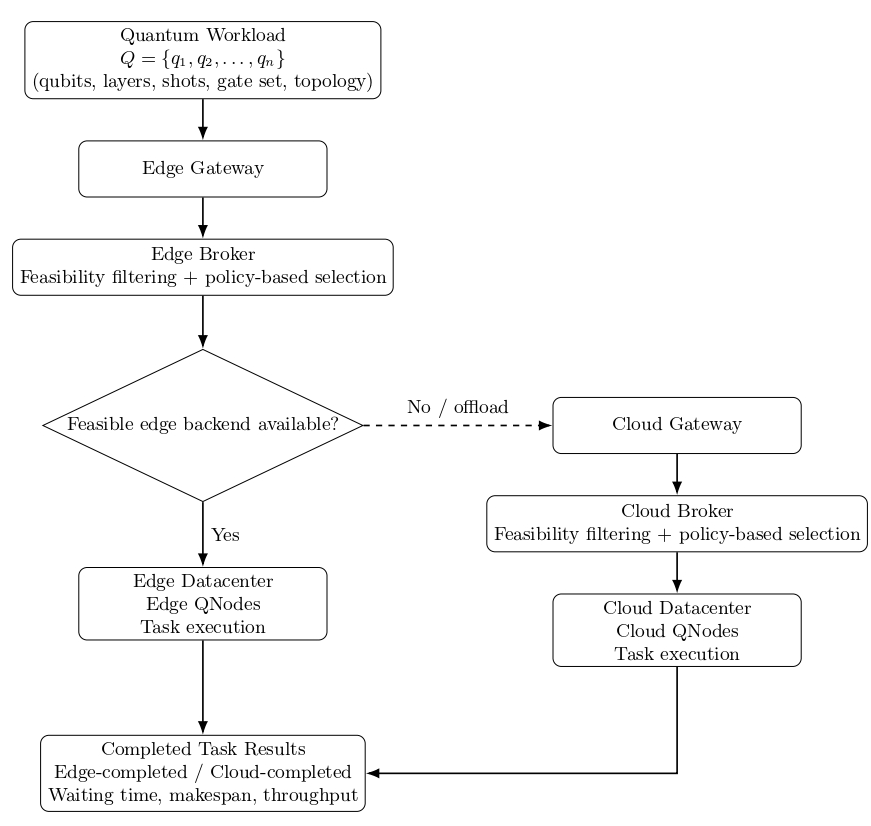
\includegraphics[width=0.85\linewidth]{Framework.png}
  % Vector alternative (page 1 of the combined PDF):
  % 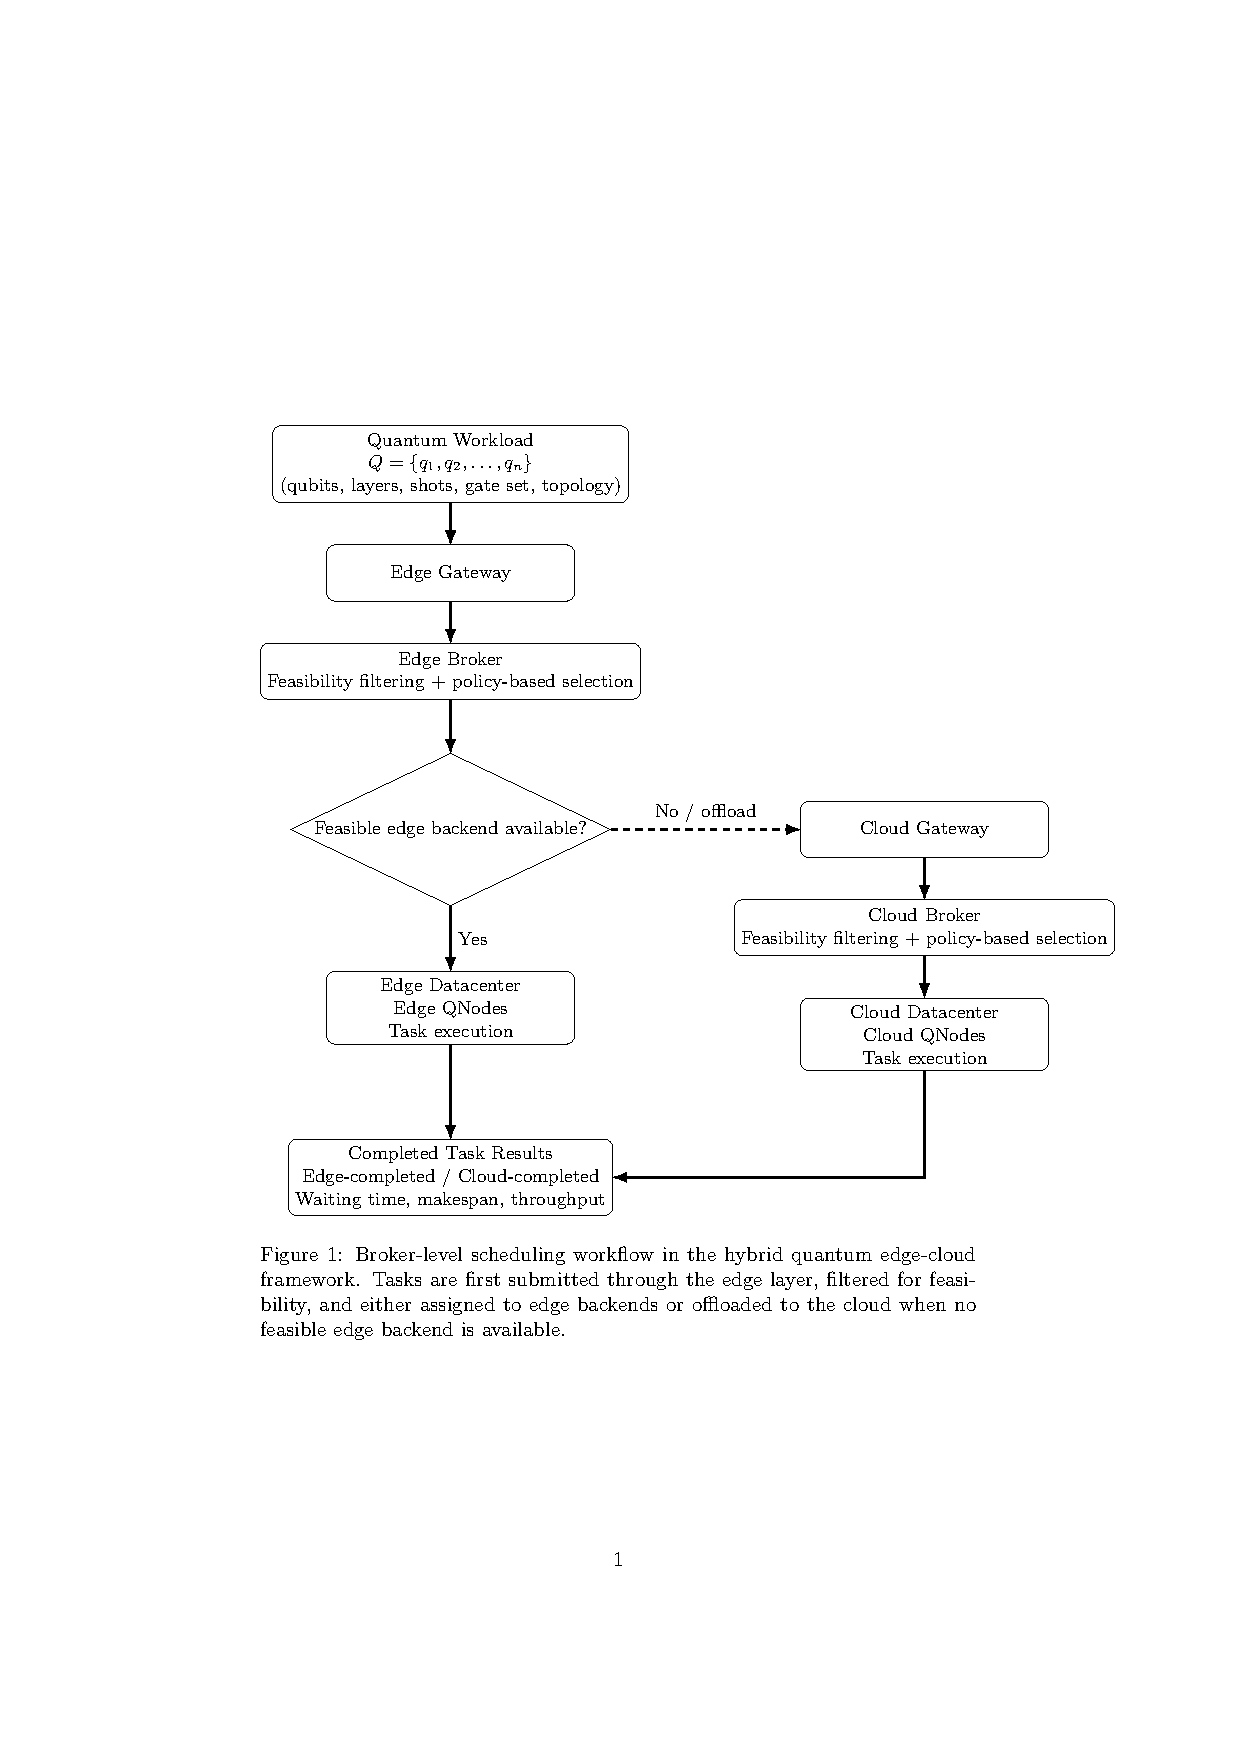
\includegraphics[width=0.85\linewidth,page=1]{Figure_Framework_and_ALgo.pdf}
  \caption{Broker-level scheduling workflow in the hybrid quantum edge--cloud
  system, illustrating edge-first routing with cloud fallback and
  feasibility-aware backend selection.}
  \label{fig:framework}
\end{figure}

\subsection{Quantum task model}
Let $Q = \{q_1, q_2, \ldots, q_n\}$ be the set of submitted quantum tasks. Each
task $q_i$ is defined by five execution-related attributes: $u_i$, the number of
qubits required; $L_i$, the number of circuit layers; $S_i$, the number of shots
required; $G_i$, the required gate set; and $T_i$, the required qubit topology.
These properties are modelled in the simulator as a \texttt{QTask} object, which
also records submission time, execution start time, finish time, wall-clock
residence time, and execution cost. The parameterisation reflects the structure
of representative near-term workloads: variational algorithms such as QAOA and
the wider family of variational quantum algorithms
\cite{farhi2014, cerezo2021} are characterised precisely by circuit depth,
shot count, and repeated submission, which is what makes execution burden a
meaningful scheduling signal. These timestamps are used to compute the
performance metrics reported later, namely waiting time, execution time,
turnaround time, makespan, and throughput.

\subsection{Feasibility-preserving scheduling stage}
Before policy-specific scheduling, a common feasibility filter is applied. For a
task $q_i$, a node $n_j$ is considered feasible if and only if
\begin{equation}
u_i \le U_j, \qquad
G_i \subseteq G_j, \qquad
\mathrm{Map}(T_i, n_j) \neq \emptyset ,
\label{eq:feasibility}
\end{equation}
where $U_j$ is the available qubit capacity on node $n_j$, $G_j$ is the supported
gate set, and $\mathrm{Map}(T_i, n_j)$ denotes an admissible topology mapping.
This feasibility step is identical across all policies and ensures that
comparisons do not confound differences in backend-selection strategy with
differences in constraint handling. The resulting feasible candidate set is
denoted $F_i$.

\subsection{Broker-side hybrid routing logic}
The implementation is based on edge-first routing. The edge broker processes
each task and assigns it to a feasible edge backend where possible. Tasks that
cannot be scheduled at the edge are offloaded to the cloud layer, where they are
resubmitted and reinserted using the same policy-specific logic, eliminating the
need for additional offloading. This realises a two-layer routing framework in
which the edge acts as the primary execution tier and the cloud as a fallback.

\subsection{Compared scheduling policies}

\subsubsection{Lottery baseline}
\Lottery{} is a stochastic baseline that chooses a backend from the feasible
candidate set $F_i$ using weighted random sampling. Ticket weights are
determined according to normalised Quantum Volume and CLOPS. Because selection
relies on unseeded randomness, \Lottery{} is non-deterministic and exhibits
run-to-run variance. It therefore serves as a capability-weighted stochastic
baseline.

\subsubsection{FCFS / first-feasible policy}
\FCFS{} performs deterministic first-feasible assignment,
\begin{equation}
n_i^{*} = \mathrm{first}(F_i).
\label{eq:fcfs}
\end{equation}
It is the simplest possible baseline and uses only feasibility ordering, with no
regard for load or capability.

\subsubsection{LoadAware policy}
\LoadAware{} selects the feasible backend with minimum predicted load,
\begin{align}
\ell_j &= r_j + w_j, \label{eq:load}\\
n_i^{*} &= \arg\min_{n_j \in F_i} \ell_j , \label{eq:loadaware}
\end{align}
where $r_j$ and $w_j$ denote the number of running and queued tasks,
respectively. Ties are broken deterministically. This policy implements simple
load balancing but does not account for execution complexity or backend
capability.

\subsection{Proposed policy: QCLAR}
\QCLAR{} (Quantum Capability and Load-Aware Routing) extends \LoadAware{} by
incorporating execution burden and backend capability. For each feasible node
$n_j \in F_i$, the composite score is defined as
\begin{equation}
\mathrm{Score}_{\QCLAR{}}(q_i, n_j)
  = \alpha\,\hat{\ell}_j + \beta\,\hat{b}_{ij} - \gamma\,\hat{c}_j ,
\label{eq:qclar}
\end{equation}
where $\hat{\ell}_j$ is the normalised predicted load, $\hat{b}_{ij}$ is the
normalised execution burden, and $\hat{c}_j$ is the normalised backend
capability. The execution burden is estimated as
\begin{equation}
b_{ij} = \frac{L_i \times S_i}{\CLOPS_j} ,
\label{eq:burden}
\end{equation}
and capability is computed as a combination of normalised CLOPS and Quantum
Volume,
\begin{equation}
c_j = 0.5\,\widehat{\CLOPS}_j + 0.5\,\widehat{\QV}_j .
\label{eq:capability}
\end{equation}
The selected backend minimises the composite score,
\begin{equation}
n_i^{*} = \arg\min_{n_j \in F_i} \mathrm{Score}_{\QCLAR{}}(q_i, n_j).
\label{eq:qclar-select}
\end{equation}
The weights are fixed as $\alpha = 0.45$, $\beta = 0.40$, and $\gamma = 0.15$.

\subsection{Proposed policy: QCLAAR}
\QCLAAR{} extends \QCLAR{} by incorporating an aging-inspired queue-pressure
term,
\begin{equation}
\mathrm{Score}_{\QCLAAR{}}(q_i, n_j)
  = \alpha\,\hat{\ell}_j + \beta\,\hat{b}_{ij} - \gamma\,\hat{c}_j
  + \lambda\,\hat{a}_j ,
\label{eq:qclaar}
\end{equation}
where $\hat{a}_j$ represents the normalised queue pressure derived from the
waiting-list size. The weights are set as $\alpha = 0.40$, $\beta = 0.30$,
$\gamma = 0.15$, and $\lambda = 0.15$. This formulation is sensitive to queue
build-up without losing the ability to make capability-driven decisions.

The weight parameters were selected empirically to balance load sensitivity,
execution complexity, and backend capability. Greater emphasis is placed on load
and execution burden in order to avoid queue accumulation, while capability is
included with a lower weight so that it influences backend selection without
dominating the decision. The same weighting structure is retained in both
\QCLAR{} and \QCLAAR{} to preserve a like-for-like comparative assessment.
Figure~\ref{fig:pipeline} summarises the internal decision-making pipelines of
\LoadAware{}, \QCLAR{}, and \QCLAAR{}.

\begin{figure}[htbp]
  \centering
  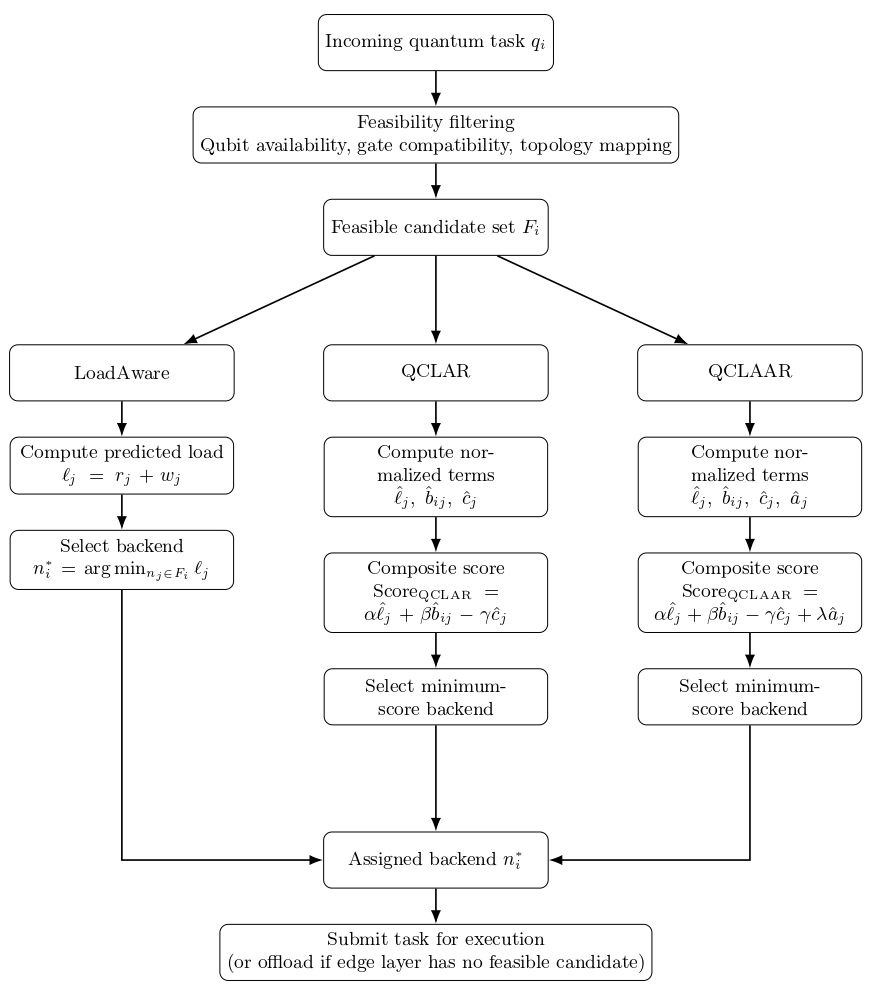
\includegraphics[width=0.85\linewidth]{flow.png}
  % Vector alternative (page 2 of the combined PDF):
  % \includegraphics[width=0.85\linewidth,page=2]{Figure_Framework_and_ALgo.pdf}
  \caption{Decision pipeline of the compared scheduling policies, showing the
  progression from feasibility filtering to load-aware and capability-aware
  scoring mechanisms.}
  \label{fig:pipeline}
\end{figure}

\subsection{Pseudocode summary}
The scoring functions are defined formally in
Equations~\eqref{eq:fcfs}--\eqref{eq:qclaar}. Algorithm~\ref{alg:broker}
summarises the common broker execution flow, and Algorithm~\ref{alg:select}
summarises the policy-specific backend-selection logic.

\begin{algorithm}[htbp]
\caption{Common broker scheduling flow}
\label{alg:broker}
\begin{algorithmic}[1]
\Require Pending task set $Q$; broker layer $\in \{\text{edge}, \text{cloud}\}$;
         policy $\pi$
\ForAll{$q_i \in Q$}
  \State Construct feasible candidate set $F_i$ using the qubit, gate-set, and
         topology constraints of Eq.~\eqref{eq:feasibility}
  \If{$F_i = \emptyset$}
    \If{broker is at the edge layer}
      \State Offload $q_i$ to the cloud layer
    \Else
      \State Mark $q_i$ as unschedulable
    \EndIf
  \Else
    \State $n_i^{*} \gets \textsc{SelectBackend}(q_i, F_i, \pi)$
    \State Submit $q_i$ to backend $n_i^{*}$
    \State Update the predicted load of $n_i^{*}$ (if applicable)
  \EndIf
\EndFor
\end{algorithmic}
\end{algorithm}

\begin{algorithm}[htbp]
\caption{Policy-specific backend selection}
\label{alg:select}
\begin{algorithmic}[1]
\Function{SelectBackend}{$q_i$, $F_i$, $\pi$}
  \If{$\pi = \FCFS{}$}
    \State \Return $\mathrm{first}(F_i)$
  \ElsIf{$\pi = \Lottery{}$}
    \State \Return weighted random sample from $F_i$ with tickets
           $\propto \hat{c}_j$
  \ElsIf{$\pi = \LoadAware{}$}
    \State \Return $\arg\min_{n_j \in F_i} \ell_j$
  \ElsIf{$\pi = \QCLAR{}$}
    \State \Return $\arg\min_{n_j \in F_i}
           \mathrm{Score}_{\QCLAR{}}(q_i, n_j)$
  \ElsIf{$\pi = \QCLAAR{}$}
    \State \Return $\arg\min_{n_j \in F_i}
           \mathrm{Score}_{\QCLAAR{}}(q_i, n_j)$
  \EndIf
\EndFunction
\end{algorithmic}
\end{algorithm}

All scoring functions are evaluated per candidate backend and incur constant
time overhead.

\subsection{Methodological remarks}
All policies share a common feasibility stage and hybrid routing structure,
which makes them directly comparable. Matched broker implementations at both the
edge and cloud layers permit homogeneous assessment of hybrid execution regimes.
The computational complexity of every policy is proportional to the number of
feasible backends, and \QCLAR{} and \QCLAAR{} add only a small constant overhead
for score computation. Given the small number of candidates per decision, this
overhead is negligible in practice.

%=====================================================================
\section{Experimental Setup}
\label{sec:setup}
%=====================================================================

\subsection{Evaluation objective}
Experiments are performed using the iQuantum simulation framework, which
provides abstractions of hybrid edge--cloud quantum computing environments. The
simulator models quantum backends abstractly in terms of qubit capacity,
execution capacity, and scheduling, while allowing broker-level control of task
routing and execution.

Using iQuantum enables scheduling policies to be evaluated in a controlled
manner over heterogeneous resource configurations without requiring access to
physical quantum hardware. This facilitates systematic comparison of scheduling
strategies across varying workload regimes. For clarity and reproducibility,
Table~\ref{tab:config} summarises the complete experimental design, system
architecture, workload, scheduling policies, and evaluation measures.

\begin{table}[htbp]
\centering
\caption{Experimental configuration summary of the hybrid quantum edge--cloud
system.}
\label{tab:config}
\small
\setlength{\tabcolsep}{5pt}
\begin{tabular}{llp{0.42\linewidth}}
\toprule
\textbf{Category} & \textbf{Parameter} & \textbf{Value / Description} \\
\midrule
Architecture        & Hybrid layers          & 1 Edge Datacenter + 1 Cloud Datacenter \\
Infrastructure      & Edge nodes             & 5 QNodes (IBM-style) \\
Infrastructure      & Cloud nodes            & 6 heterogeneous QNodes \\
Cloud capability    & CLOPS                  & $\{220, 320, 450, 700, 1000, 1400\}$ \\
Cloud capability    & Quantum Volume (QV)    & $\{32, 48, 64, 96, 128, 192\}$ \\
Workload model      & Task type              & QTask (qubits, depth, shots, gates, topology) \\
Policies            & Baselines              & FCFS, Lottery, LoadAware \\
Policies            & Proposed               & QCLAR, QCLAAR \\
Scheduling          & Feasibility filter     & Qubit capacity, gate set, topology mapping \\
Scheduling          & Offloading rule        & Edge-infeasible tasks $\rightarrow$ Cloud \\
Scenarios           & Execution modes        & No-Stress, Stress \\
Stress design       & Workload mix           & 50\% small, 30\% medium, 20\% heavy \\
Experiment control  & Workload duplication   & Disabled \\
Reproducibility     & Repetitions            & 5 runs per policy; deterministic policies confirmed stable (zero variance) \\
Metrics             & Reported               & Waiting time, makespan, throughput, execution distribution \\
\bottomrule
\end{tabular}
\end{table}

\subsection{System configuration}
The hybrid environment comprises an edge layer with low-capacity quantum
backends and a cloud layer with high-capacity systems. Edge nodes typically
provide fewer qubits and medium-scale processing power, in contrast to the large
Quantum Volume and CLOPS values of cloud backends. Whereas cloud quantum
computing offers scalable, high-performance execution, edge devices may have
limited quantum resources but permit low-latency processing. This design
reflects realistic deployment conditions. System factors such as qubit capacity
and performance metrics are chosen so as to clearly distinguish cloud and edge
capabilities, allowing scheduling policies to be evaluated under practical
heterogeneity.

\subsection{Workload datasets}
Scheduler performance is evaluated using four datasets (Set01--Set04) with
varying workload scale and complexity, drawn from the MQT Bench circuit
collection~\cite{quetschlich2023} and mapped to IBM device topologies.
Table~\ref{tab:workload} reports the task counts and topology mapping verified
directly from the simulation output; task-level detail (individual circuit
depth and shot count per task) is generated by the underlying MQT Bench
mapping pipeline and is not reproduced here. Set01 and Set02 are mapped to a
27-qubit IBM Quantum topology and are executed entirely at the edge layer.
Set03 requires the full 127-qubit topology, which no edge backend in
Table~\ref{tab:config} satisfies, so it executes entirely in the cloud. Set04
is constructed by adding 1497 edge-feasible tasks to Set03's identical 5818
cloud-bound tasks, giving a genuine mixed edge/cloud workload rather than an
independent fourth dataset. This progression makes it possible to study how a
scheduler reacts to increasing system pressure and workload heterogeneity, and
the workload design ensures coverage of edge-only, cloud-only, and mixed
execution regimes.

\begin{table}[htbp]
\centering
\caption{Workload datasets, verified from simulation output. Task counts and
the edge/cloud split are identical across all five scheduling policies
(Section~\ref{sec:regime}).}
\label{tab:workload}
\small
\begin{tabular}{lrlp{0.32\linewidth}}
\toprule
\textbf{Dataset} & \textbf{Tasks} & \textbf{Topology} & \textbf{Relation to other datasets} \\
\midrule
Set01 & 298  & 27-qubit (IBMQ) & Independent \\
Set02 & 1133 & 27-qubit (IBMQ, mapped) & Independent \\
Set03 & 5818 & 127-qubit (IBM, mapped) & Independent \\
Set04 & 7315 & Mixed (27- and 127-qubit) & Set03's 5818 tasks + 1497 additional \\
\bottomrule
\end{tabular}
\end{table}

\subsection{Stress modelling}
Two execution regimes are considered: non-stressed and stressed. The stressed
setting intensifies the burden by increasing computational load and task arrival
rates. This approach mimics real-world scenarios involving congested quantum
resources by testing scheduler robustness under strong system pressure. Stress
parameters are designed so as to induce queue build-up and resource contention
without rendering the system infeasible, allowing meaningful comparison between
policies. Because the trials compare stressed and non-stressed settings, they
isolate the influence of workload pressure on scheduling efficiency and
scalability.

\subsection{Scheduling policies}
The evaluation covers the \FCFS{}, \Lottery{}, \LoadAware{}, \QCLAR{}, and
\QCLAAR{} scheduling policies. These policies reflect progressively increasing
levels of sophistication, starting from basic feasibility-based assignment and
ending with capability-aware selection. All policies employ the same routing
logic and operate under the same feasibility restrictions, so that performance
differences can be attributed solely to the backend-selection method.

\subsection{Performance metrics}
Scheduler performance is measured using the following metrics:
\begin{itemize}
  \item \textbf{Average waiting time}: the mean delay between submission and the
        start of execution of a task.
  \item \textbf{Makespan}: the time taken to complete all tasks.
  \item \textbf{Throughput}: the number of completed tasks per unit time.
  \item \textbf{Execution distribution}: the split of completed tasks between the
        edge and cloud layers.
\end{itemize}
Together, these measures capture scheduling efficiency, system utilisation, and
resource allocation behaviour.

\subsection{Experimental procedure}
A single structure is used for all experiments, and two configurations---stressed
and non-stressed---are tested. System parameters are applied uniformly across all
scheduling policies and datasets. Every policy, including the deterministic
ones, was executed five times per dataset and condition ($5 \times 5 \times 4
\times 2 = 200$ recorded runs in total); this confirmed empirically that
\FCFS{}, \LoadAware{}, \QCLAR{}, and \QCLAAR{} return identical results on
every execution (zero variance across runs) and quantified the run-to-run
variability of \Lottery{}, for which means and standard deviations are reported
throughout. All results are recorded in CSV format and used directly to
construct the comparison tables and figures reported below; throughput is
recomputed from completed-task counts and makespan at full precision, since the
logged throughput field is rounded to four decimal places.

%=====================================================================
\section{Results and Discussion}
\label{sec:results}
%=====================================================================
This section compares scheduler performance across workload regimes and stress
levels in order to identify performance trends and policy robustness.

\subsection{Hybrid execution regimes}
\label{sec:regime}
Table~\ref{tab:regime} and Figure~\ref{fig:regime} show the distribution of task
execution across the edge and cloud layers. Execution behaviour varies
considerably between datasets. Set01 (298 tasks) and Set02 (1133 tasks) are
built from smaller circuits mapped to the 27-qubit edge backends and complete
entirely at the edge. Set03 consists of 5818 tasks requiring the full 127-qubit
topology, which no edge backend satisfies, so every task is offloaded to the
cloud. Set04 is constructed as Set03's 5818 cloud-bound tasks plus an additional
1497 edge-feasible tasks (7315 total), giving a genuine mixed regime rather than
a fourth independent workload.

This split is determined entirely by the feasibility filter of
Eq.~\eqref{eq:feasibility} and is therefore identical for every scheduling
policy: across all five policies and both stress conditions, edge- and
cloud-completed counts for a given dataset do not vary. Table~\ref{tab:regime}
is accordingly reported once rather than per policy. The composite-score
policies affect \emph{which} backend a task receives within a layer, not
\emph{which} layer it is routed to.

\begin{table}[htbp]
\centering
\caption{Execution regime across datasets, confirmed identical for all five
scheduling policies under both stress conditions.}
\label{tab:regime}
\begin{tabular}{lrrp{0.3\linewidth}}
\toprule
\textbf{Dataset} & \textbf{Edge completed} & \textbf{Cloud completed} & \textbf{Regime} \\
\midrule
Set01 & 298  & 0    & Edge-only \\
Set02 & 1133 & 0    & Edge-dominant \\
Set03 & 0    & 5818 & Cloud-only \\
Set04 & 1497 & 5818 & Mixed hybrid (Set03's cloud tasks + 1497 edge tasks) \\
\bottomrule
\end{tabular}
\end{table}

\begin{figure}[htbp]
  \centering
  \begin{subfigure}[b]{0.49\linewidth}
    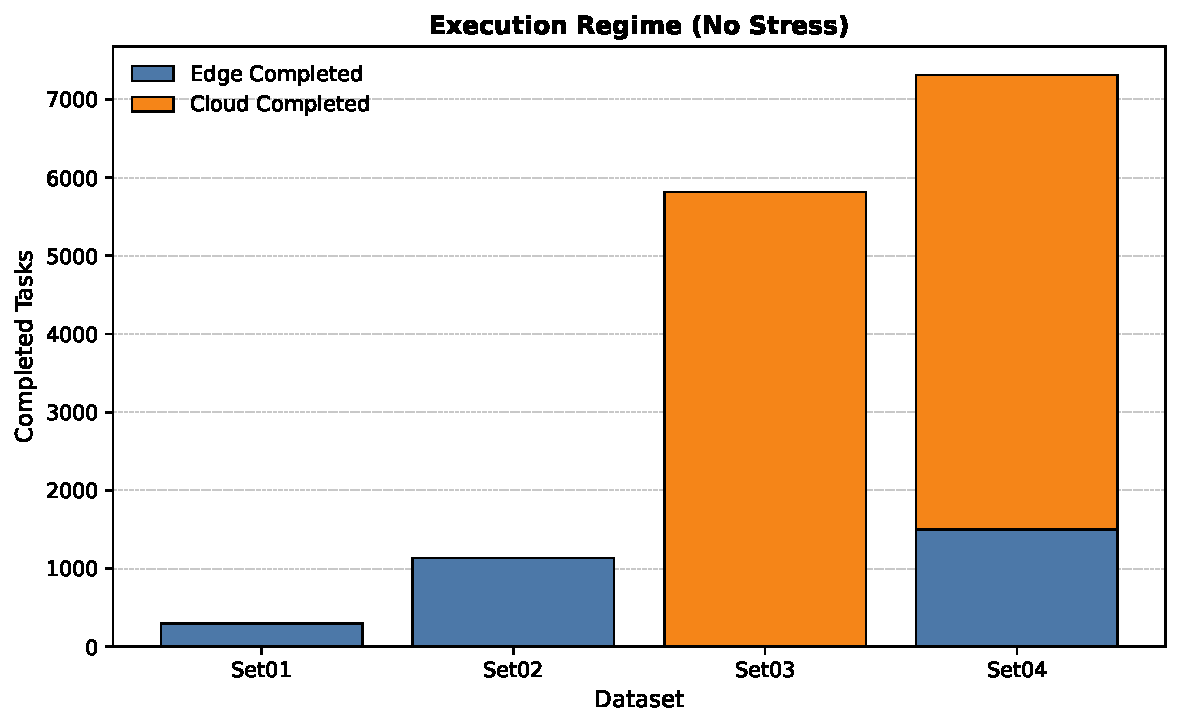
\includegraphics[width=\linewidth]{Figure1_execution_regime_no_stress.pdf}
    \caption{No-stress condition}
    \label{fig:regime-nostress}
  \end{subfigure}
  \hfill
  \begin{subfigure}[b]{0.49\linewidth}
    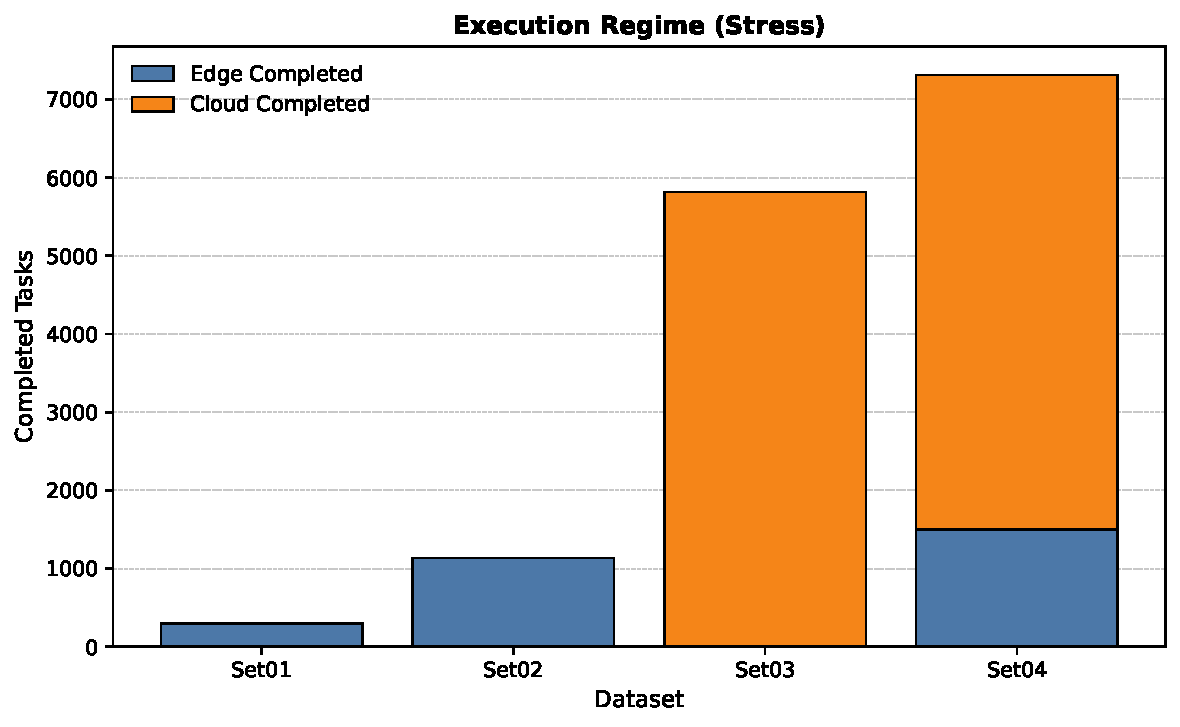
\includegraphics[width=\linewidth]{Figure1_execution_regime_stress.pdf}
    \caption{Stress condition}
    \label{fig:regime-stress}
  \end{subfigure}
  \caption{Distribution of completed tasks across the edge and cloud layers. The
  four datasets expose edge-only, cloud-dominant, and mixed hybrid execution
  regimes.}
  \label{fig:regime}
\end{figure}

\subsection{Average waiting time analysis}
Figures~\ref{fig:wait-nostress} and~\ref{fig:wait-stress} compare the average
waiting times of the scheduling policies across all datasets under no-stress and
stress scenarios. \FCFS{} exhibits the longest waiting times in every condition,
which is expected given that it accounts for neither load imbalance nor backend
capacity. \Lottery{} reduces waiting time substantially relative to \FCFS{} by
probabilistically favouring more capable backends, but its stochastic selection
leaves it consistently behind the deterministic capability-aware policies.
\LoadAware{} achieves large reductions by prioritising less congested backends,
confirming the value of load balancing as a first-order signal.

The margin between \LoadAware{} and the proposed policies is strongly
scale-dependent, and this is the central observation of the waiting-time
results. On the two smaller datasets the three are effectively indistinguishable:
on Set01, \QCLAR{} and \QCLAAR{} improve on \LoadAware{} by only 0.8\%
(20.67K versus 20.83K), and on Set02 \LoadAware{} is in fact marginally ahead
(179.59K versus 179.79K, a difference of 0.1\%). Differences of this magnitude
should not be read as a performance ordering. On Set03 and Set04, however, the
gap widens sharply: \QCLAAR{} reduces waiting time relative to \LoadAware{} by
26.0\% and 25.8\% respectively under no stress, and by 28.1\% and 24.6\% under
stress. The interpretation is that when the feasible candidate set is
homogeneous and lightly loaded, predicted load alone is a sufficient statistic
for backend selection; execution burden and capability only begin to
discriminate once tasks are large enough, and backends heterogeneous enough,
that a load-balanced assignment can still be a poor one.

Under stress (Table~\ref{tab:wait}) every policy degrades, but the proposed
policies hold the best value in all four datasets, with \QCLAAR{} lowest on
Set03 and Set04.

\begin{table}[htbp]
\centering
\caption{Average waiting time ($\mathrm{K} = 10^{3}$, $\mathrm{M} = 10^{6}$),
computed directly from five independent simulation runs per policy, dataset,
and condition. Lottery values are mean $\pm$ sample standard deviation over the
five runs; FCFS, LoadAware, QCLAR, and QCLAAR returned identical results on
every run (zero variance) and are reported as single values. Best value per
column is shown in bold.}
\label{tab:wait}
\small
\setlength{\tabcolsep}{5pt}
\begin{tabular}{lrrrr}
\multicolumn{5}{c}{\textit{(a) No-stress condition}} \\
\toprule
\textbf{Algorithm} & \textbf{Set01} & \textbf{Set02} & \textbf{Set03} & \textbf{Set04} \\
\midrule
FCFS      & 97.84K            & 833.15K            & 122.20M            & 97.55M \\
Lottery   & 36.70$\pm$1.64K   & 321.88$\pm$16.59K  & 7.13$\pm$0.02M     & 5.83$\pm$0.04M \\
LoadAware & 20.83K            & \textbf{179.59K}   & 9.49M              & 7.63M \\
QCLAR     & \textbf{20.67K}   & 179.79K            & 7.11M              & 5.73M \\
QCLAAR    & \textbf{20.67K}   & 179.79K            & \textbf{7.02M}     & \textbf{5.66M} \\
\bottomrule
\addlinespace[1.2ex]
\multicolumn{5}{c}{\textit{(b) Stress condition}} \\
\toprule
\textbf{Algorithm} & \textbf{Set01} & \textbf{Set02} & \textbf{Set03} & \textbf{Set04} \\
\midrule
FCFS      & 246.70K           & 2.68M              & 263.95M            & 202.03M \\
Lottery   & 93.81$\pm$8.04K   & 1.00$\pm$0.06M     & 15.48$\pm$0.09M    & 12.08$\pm$0.10M \\
LoadAware & 57.79K            & 633.45K            & 21.17M             & 15.41M \\
QCLAR     & \textbf{56.46K}   & \textbf{629.12K}   & 15.32M             & 11.85M \\
QCLAAR    & \textbf{56.46K}   & \textbf{629.12K}   & \textbf{15.23M}    & \textbf{11.62M} \\
\bottomrule
\end{tabular}
\end{table}

\begin{figure}[htbp]
  \centering
  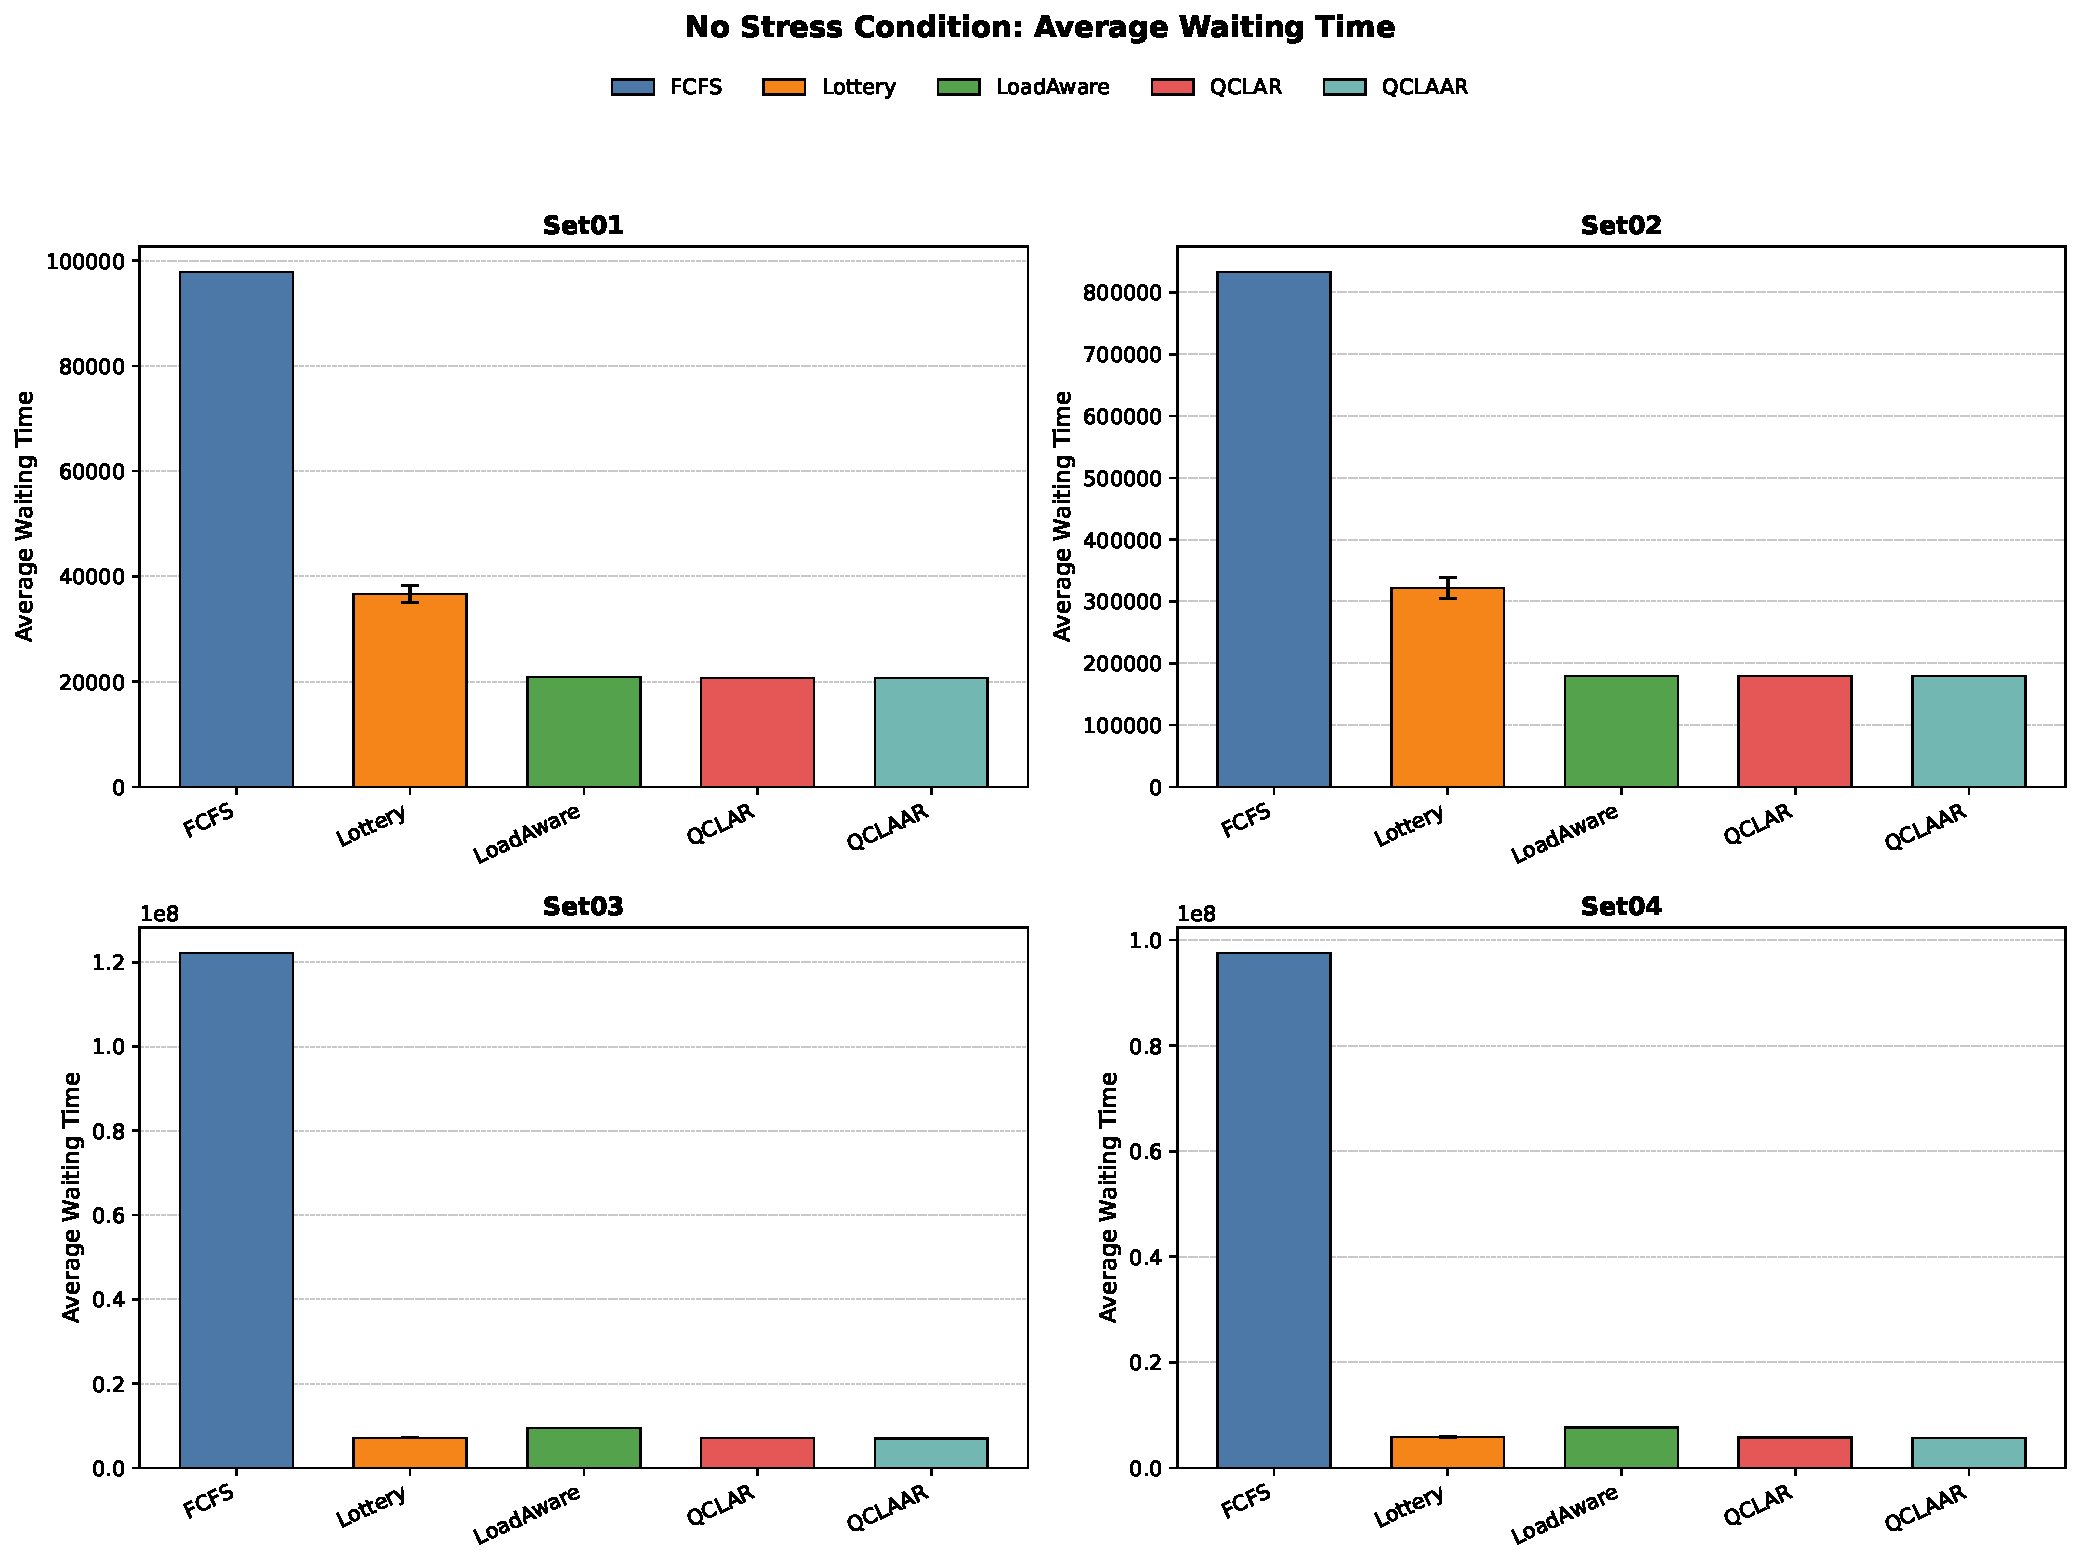
\includegraphics[width=0.95\linewidth]{Figure2_no_stress_waiting_time.pdf}
  \caption{Average waiting time under no-stress conditions.}
  \label{fig:wait-nostress}
\end{figure}

\begin{figure}[htbp]
  \centering
  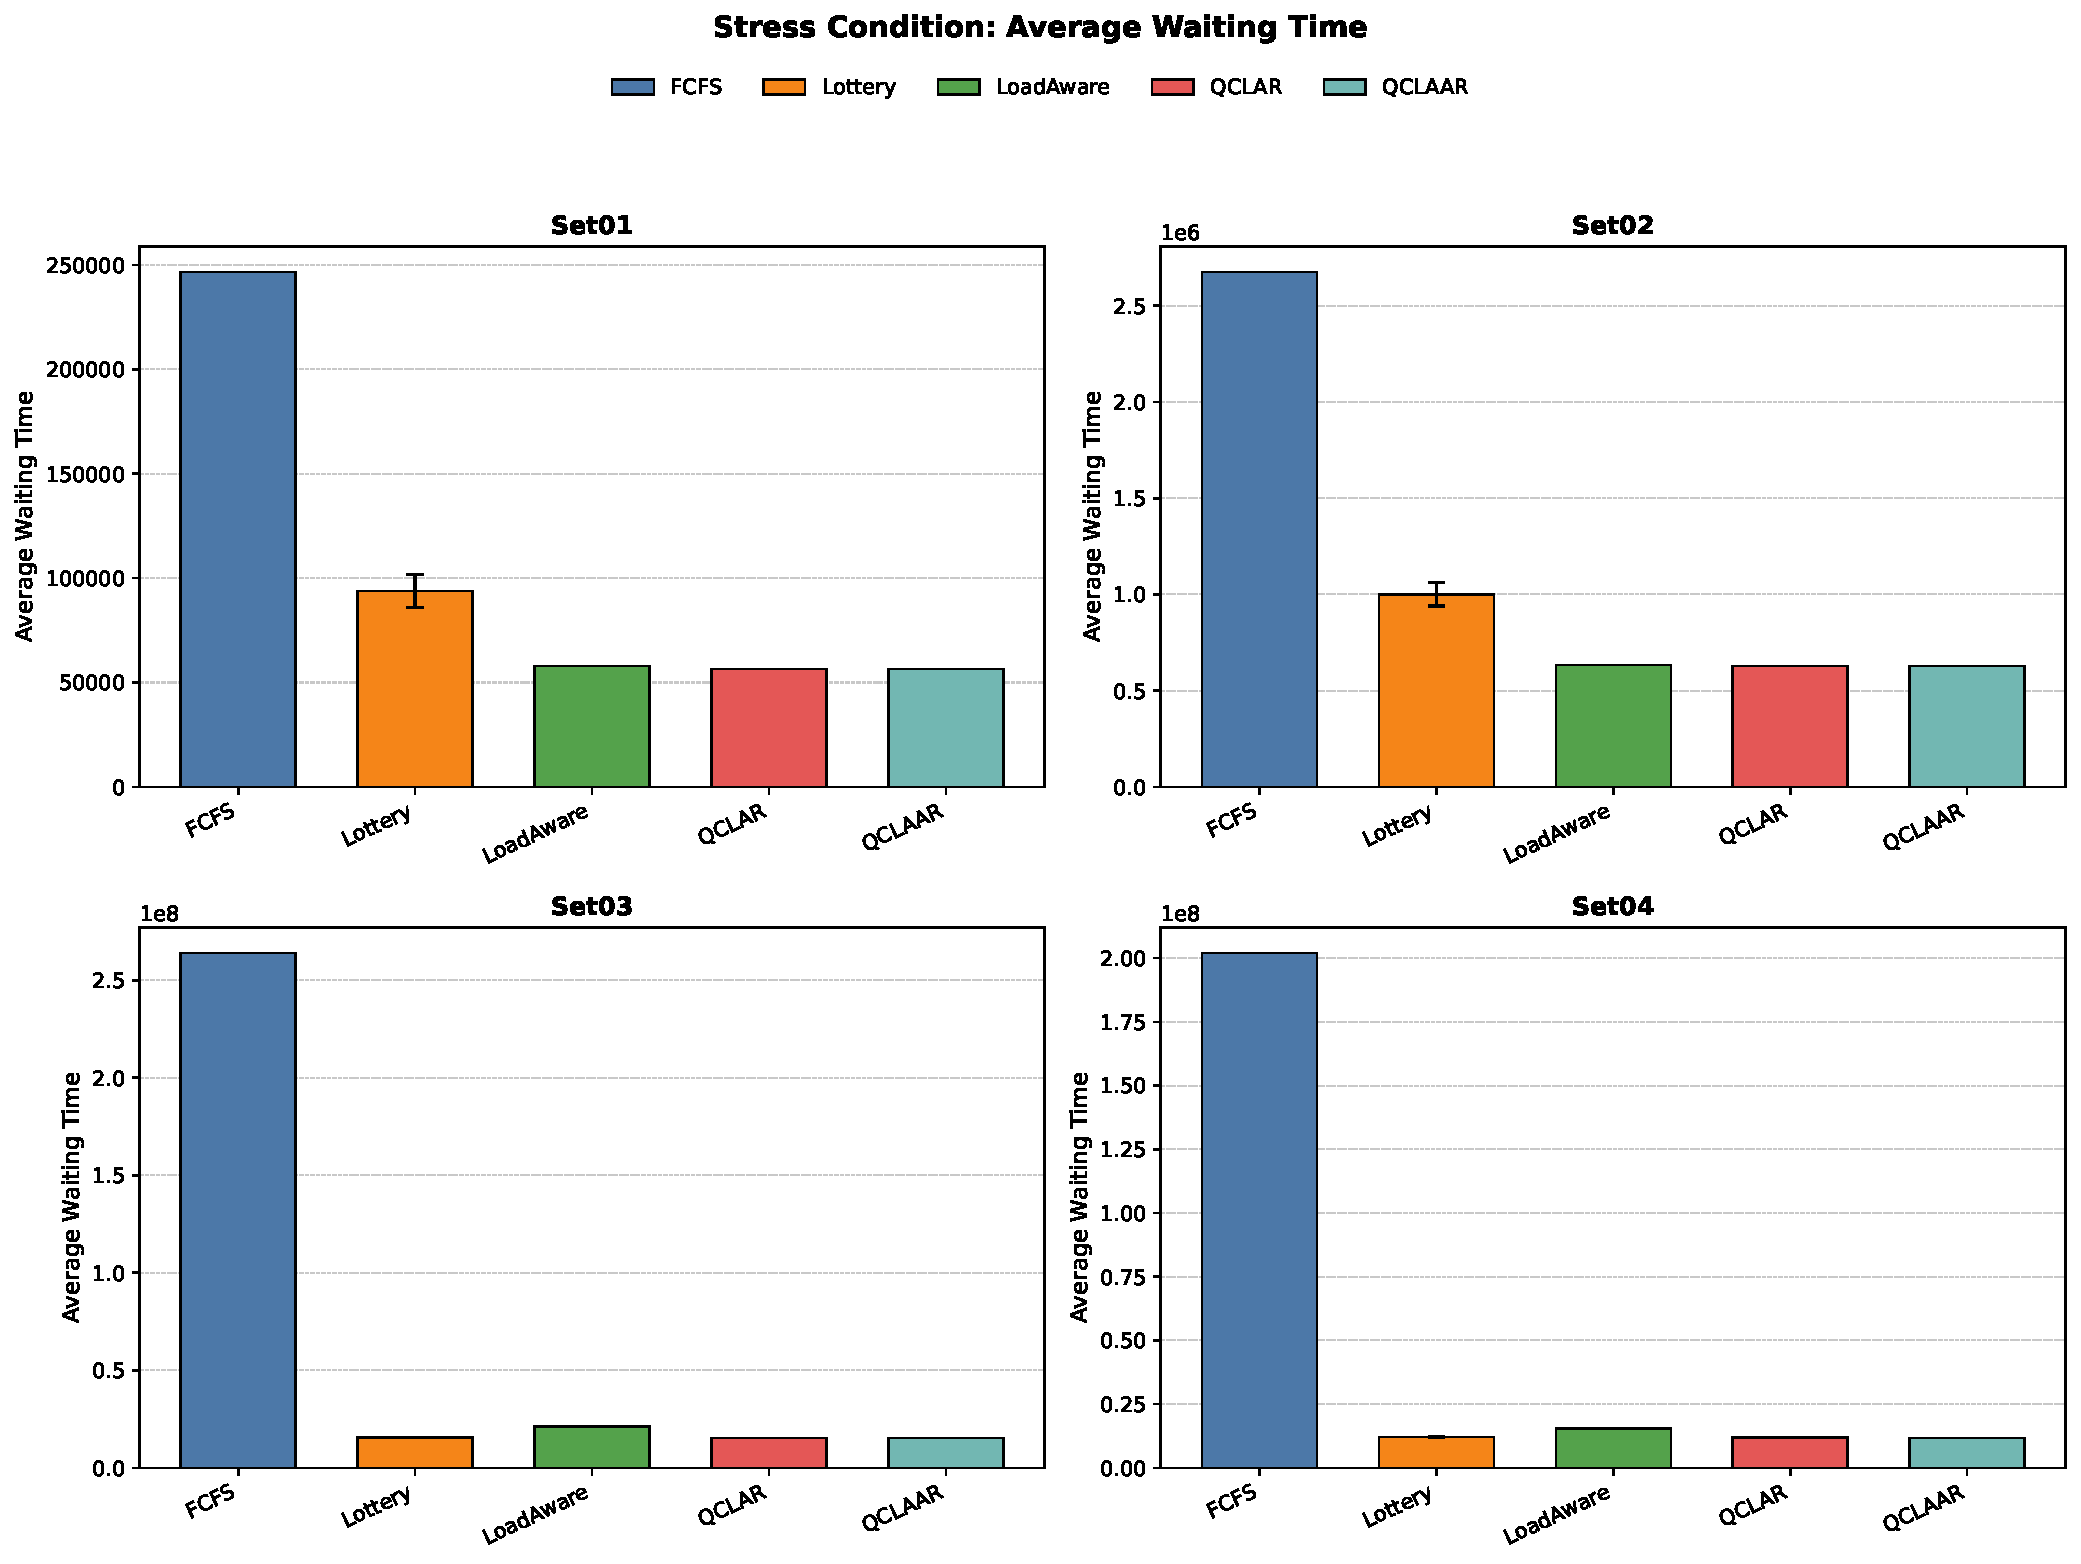
\includegraphics[width=0.95\linewidth]{Figure5_stress_waiting_time.pdf}
  \caption{Average waiting time under stress conditions.}
  \label{fig:wait-stress}
\end{figure}

\subsection{Makespan analysis}
Figures~\ref{fig:mksp-nostress} and~\ref{fig:mksp-stress} show the makespan of
each scheduling policy. \FCFS{} again exhibits the longest makespan in every
condition, consistent with the waiting-time trends. The remaining ordering is
less uniform than for waiting time, and the differences are informative.

A feature of Table~\ref{tab:makespan} worth explaining directly is that, under
no stress, every policy's Set03 and Set04 makespan agree to within 0.01 time
units on values of order $10^{7}$--$10^{8}$ (for example, \FCFS{} gives
244\,977\,497.04 on Set03 against 244\,977\,497.05 on Set04). This is a
consequence of how the two datasets relate (Section~\ref{sec:setup}): Set04
adds 1497 edge-feasible tasks to Set03's identical 5818 cloud-bound tasks. Under
no stress those extra tasks complete quickly and in parallel at the edge, well
before the cloud queue drains, so they do not extend the point at which the
last task finishes and the two datasets share a makespan. They do, however,
pull the \emph{mean} waiting time down for Set04 relative to Set03, since that
average is taken over all completed tasks including the fast edge ones ---
consistent with Table~\ref{tab:wait}, where every policy's Set04 waiting time is
lower than its Set03 waiting time. Under stress the coincidence breaks down (for
instance \FCFS{} gives 529.58M on Set03 against 511.01M on Set04): the edge
layer itself becomes congested under the stress workload mix, so the extra
tasks are no longer negligible to the critical path.

Under no stress, \QCLAAR{} achieves the lowest makespan on Set01, Set03, and
Set04, but \LoadAware{} is best on Set02 (451.40K against 469.16K for the
proposed policies, a 3.9\% advantage). Under stress the picture is more mixed
still: \Lottery{} records the lowest makespan on Set01 (242.20K) and Set03
(36.06M), while \QCLAR{} and \QCLAAR{} lead on Set02 and \QCLAR{} on Set04.
\Lottery{}'s competitiveness here deserves comment rather than dismissal. Its
tickets are weighted by normalised Quantum Volume and CLOPS, so it is already a
capability-biased policy; what it lacks is load and execution-burden awareness.
Under stress, when queues are long at every candidate backend, the value of
load information falls and capability weighting alone captures most of the
available benefit. The cost is reproducibility, examined in
Section~\ref{sec:variability}: the Set01 stress figure of 242.20K carries a
standard deviation of 35.56K across five runs, so a single \Lottery{} execution
may return a makespan anywhere from roughly 207K to 278K.

Across the large datasets the consistent result is the margin over
\LoadAware{}, which is substantial in every condition --- 60.5\% on Set03 and
60.5\% on Set04 under no stress, and 57.4\% and 63.4\% under stress. Load
balancing alone leaves considerable makespan on the table once workloads are
heterogeneous.

\begin{table}[htbp]
\centering
\caption{Makespan ($\mathrm{K} = 10^{3}$, $\mathrm{M} = 10^{6}$), computed
directly from five independent simulation runs per policy, dataset, and
condition. Lottery values are mean $\pm$ sample standard deviation over the
five runs; the deterministic policies returned identical results on every run
and are reported as single values. Best value per column is shown in bold.}
\label{tab:makespan}
\small
\setlength{\tabcolsep}{5pt}
\begin{tabular}{lrrrr}
\multicolumn{5}{c}{\textit{(a) No-stress condition}} \\
\toprule
\textbf{Algorithm} & \textbf{Set01} & \textbf{Set02} & \textbf{Set03} & \textbf{Set04} \\
\midrule
FCFS      & 197.28K           & 1.72M               & 244.98M         & 244.98M \\
Lottery   & 92.00$\pm$10.03K  & 886.99$\pm$164.84K  & 16.26$\pm$0.45M & 16.74$\pm$0.62M \\
LoadAware & 63.27K            & \textbf{451.40K}    & 39.90M          & 39.90M \\
QCLAR     & \textbf{56.94K}   & 469.16K             & 16.92M          & 16.92M \\
QCLAAR    & \textbf{56.94K}   & 469.16K             & \textbf{15.76M} & \textbf{15.76M} \\
\bottomrule
\addlinespace[1.2ex]
\multicolumn{5}{c}{\textit{(b) Stress condition}} \\
\toprule
\textbf{Algorithm} & \textbf{Set01} & \textbf{Set02} & \textbf{Set03} & \textbf{Set04} \\
\midrule
FCFS      & 452.67K                    & 4.46M            & 529.58M                  & 511.01M \\
Lottery   & \textbf{242.20$\pm$35.56K} & 2.64$\pm$0.88M   & \textbf{36.06$\pm$1.19M} & 35.63$\pm$2.12M \\
LoadAware & 290.88K                    & 2.90M            & 90.32M                   & 89.61M \\
QCLAR     & 261.80K                    & \textbf{2.61M}   & 37.42M                   & \textbf{31.79M} \\
QCLAAR    & 261.80K                    & \textbf{2.61M}   & 38.44M                   & 32.79M \\
\bottomrule
\end{tabular}
\end{table}

\begin{figure}[htbp]
  \centering
  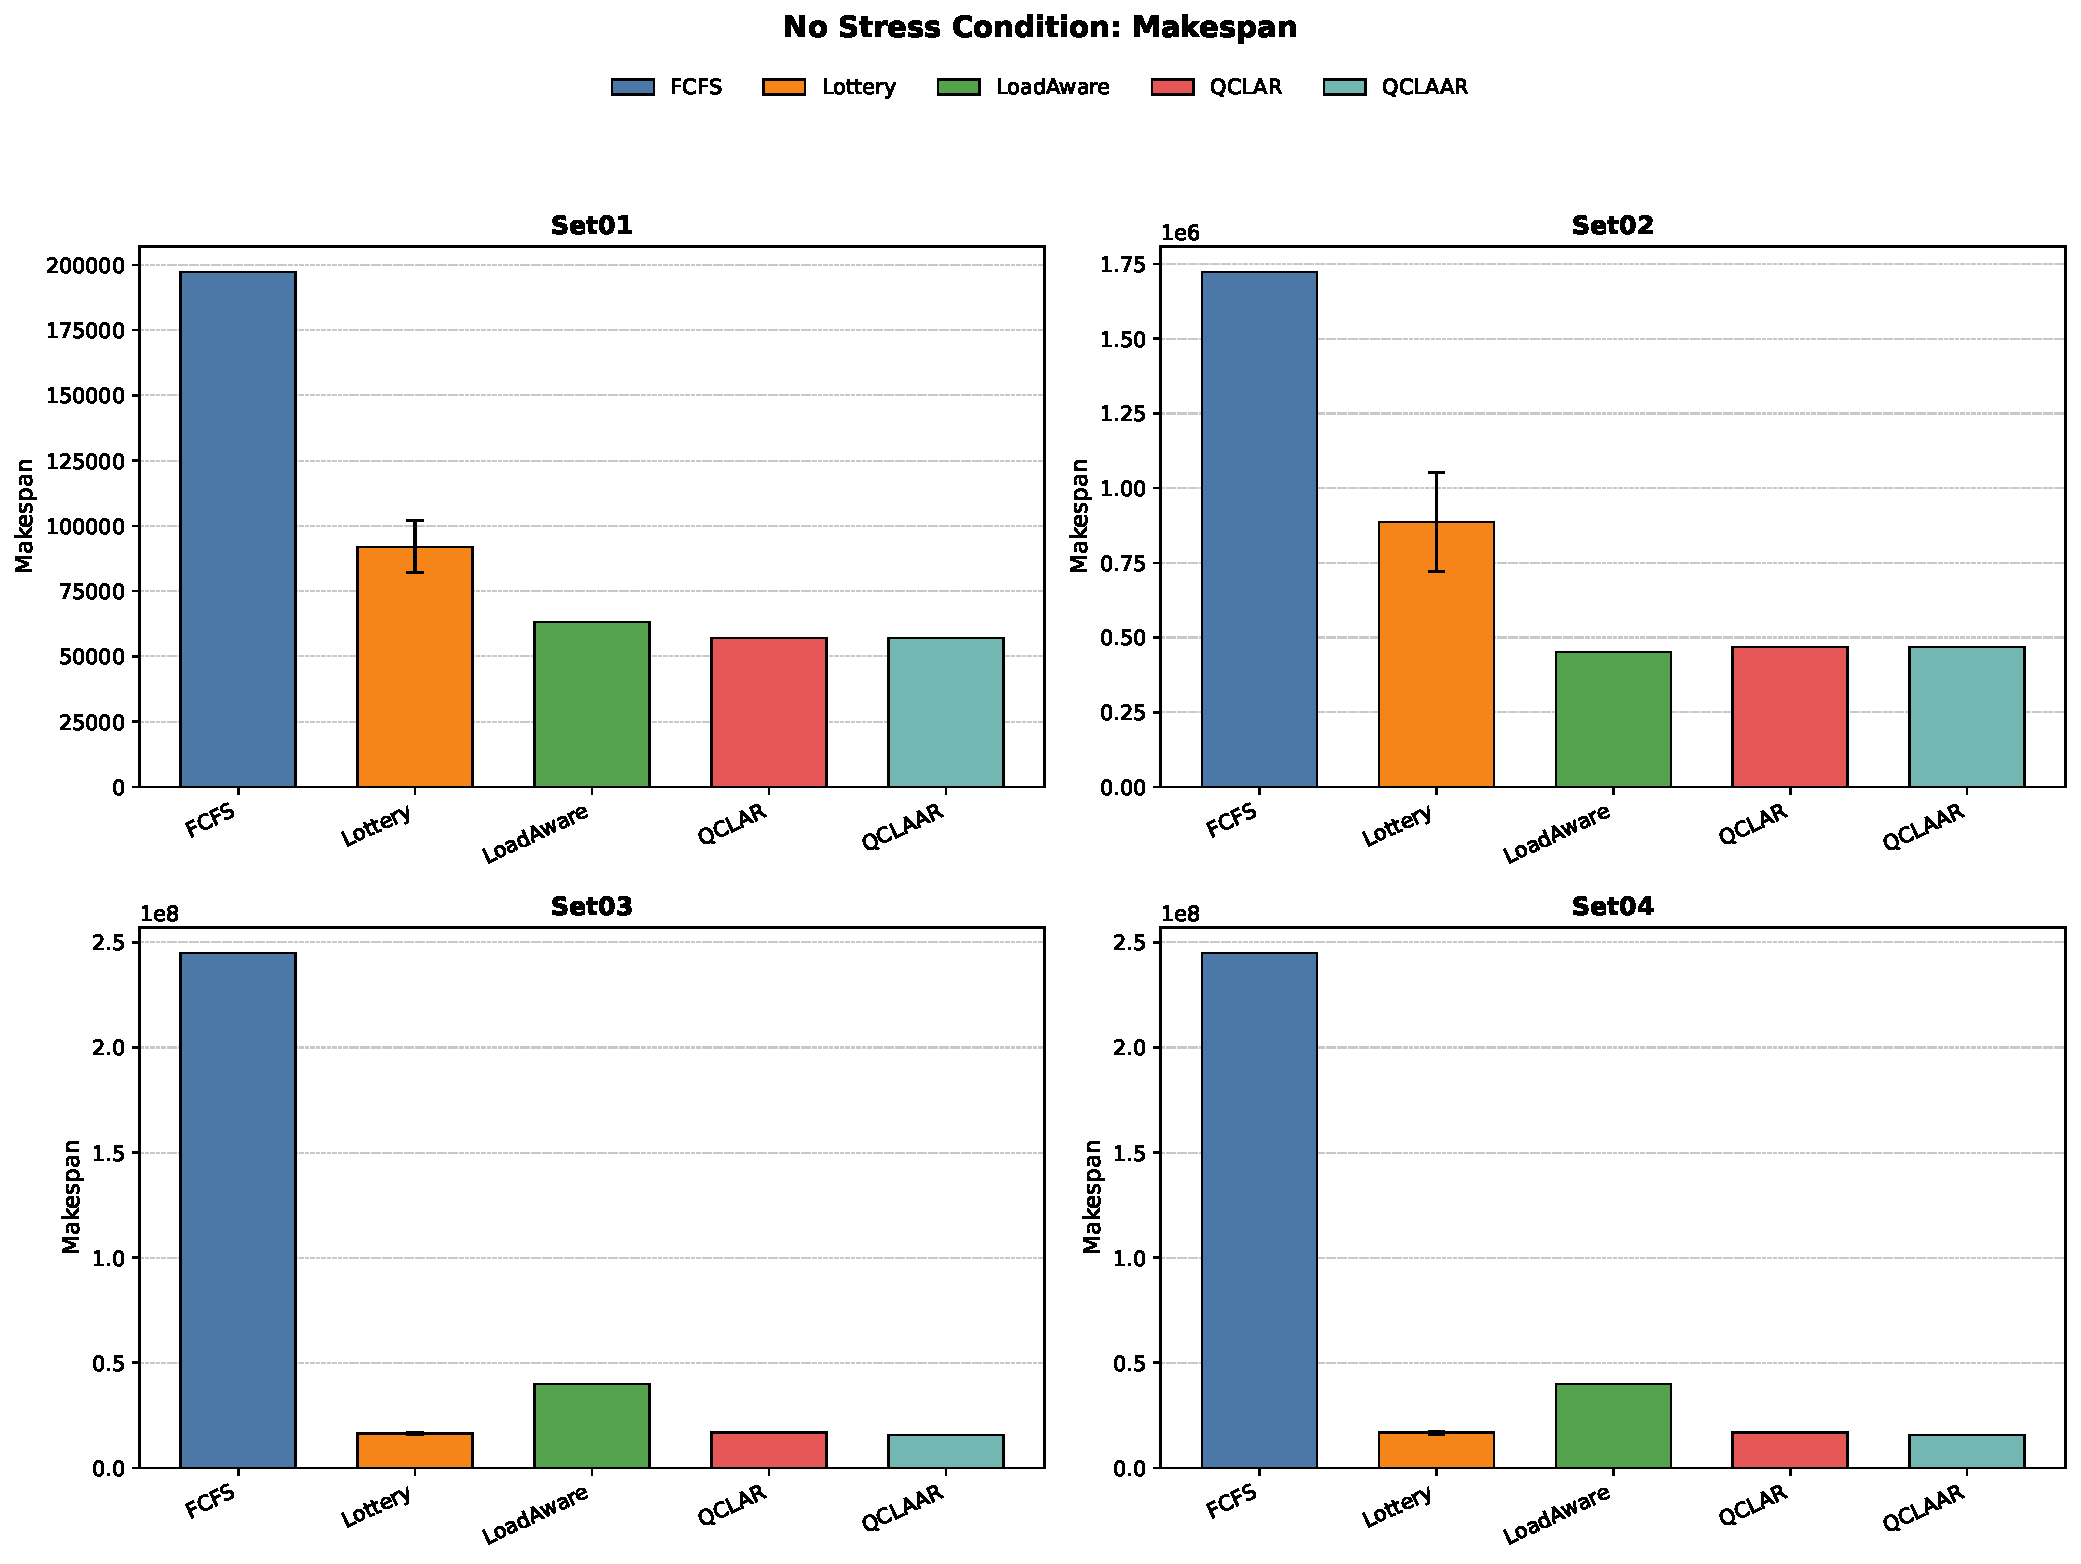
\includegraphics[width=0.95\linewidth]{Figure3_no_stress_makespan.pdf}
  \caption{Makespan under no-stress conditions.}
  \label{fig:mksp-nostress}
\end{figure}

\begin{figure}[htbp]
  \centering
  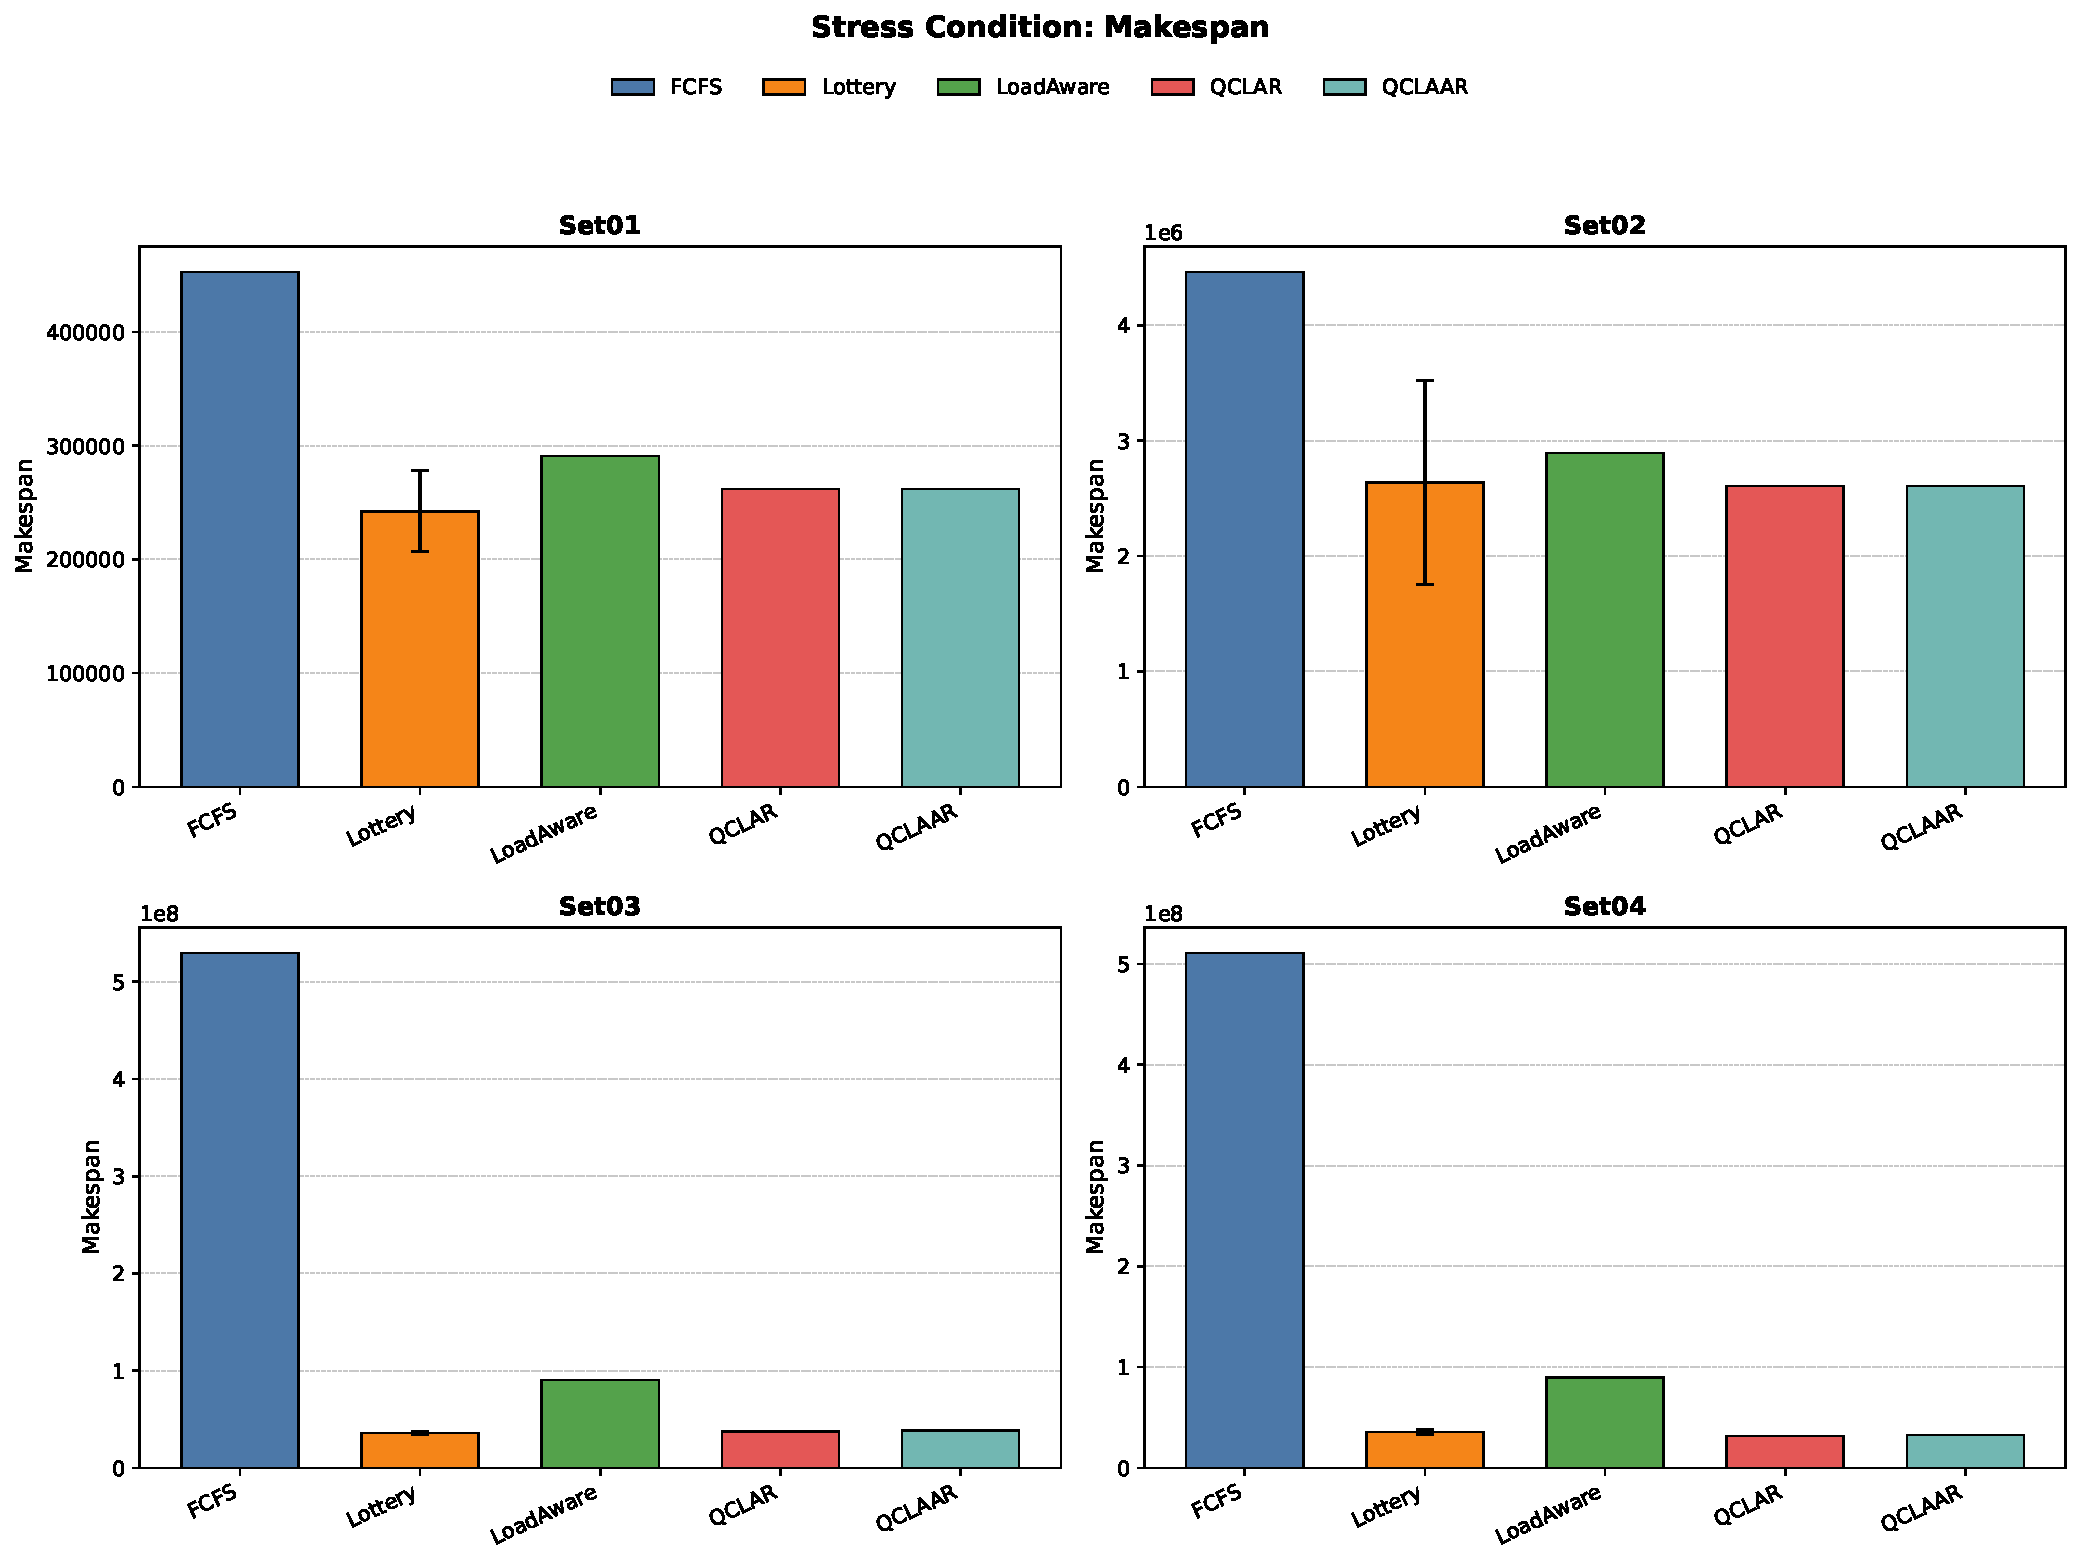
\includegraphics[width=0.95\linewidth]{Figure6_stress_makespan.pdf}
  \caption{Makespan under stress conditions.}
  \label{fig:mksp-stress}
\end{figure}

\subsection{Throughput analysis}
Table~\ref{tab:throughput} reports throughput computed as
$\mathrm{total\ completed} / \mathrm{makespan}$ at full precision from the
underlying simulation output; the logged throughput field, rounded to four
decimal places, is indistinguishable from zero for Set03 and Set04 and is not
used directly. Figures~\ref{fig:thr-nostress} and~\ref{fig:thr-stress} show the
same trends graphically. \FCFS{} achieves the lowest throughput throughout,
consistent with its waiting-time and makespan behaviour.

At full precision the ordering is clearer than the raw simulator output
suggests, and largely mirrors the waiting-time result. Under no stress, \QCLAR{}
or \QCLAAR{} attain the highest throughput on three of four datasets ---
\QCLAR{} on Set01, \QCLAAR{} on Set03 and Set04 --- with \LoadAware{} again the
exception on Set02. Under stress the picture matches the makespan result:
\Lottery{} leads on Set01, Set02, and Set03, while \QCLAR{} leads on Set04. As
with makespan, \Lottery{}'s stress-condition lead should be read against its
run-to-run variance (Section~\ref{sec:variability}): its Set02 throughput of
$0.469 \times 10^{-3}$ carries a standard deviation of
$0.151 \times 10^{-3}$, over 30\% of the mean.

Taken together with Sections 5.2 and 5.3, the proposed policies win 16 of the
24 metric--dataset--condition combinations across waiting time, makespan, and
throughput; \LoadAware{} wins the 3 combinations on Set02 under no stress, and
\Lottery{} wins the remaining 5, all under stress on makespan or throughput.

\begin{table}[htbp]
\centering
\caption{Throughput ($\times 10^{-3}$ tasks per unit time), recomputed as
total completed tasks divided by makespan at full precision from the five
underlying simulation runs per policy, dataset, and condition (the raw
simulator log rounds this field to four decimal places, which is insufficient
to resolve Set03--Set04). Lottery values are mean $\pm$ sample standard
deviation. Best value per column is shown in bold.}
\label{tab:throughput}
\small
\setlength{\tabcolsep}{6pt}
\begin{tabular}{lrrrr}
\multicolumn{5}{c}{\textit{(a) No-stress condition}} \\
\toprule
\textbf{Algorithm} & \textbf{Set01} & \textbf{Set02} & \textbf{Set03} & \textbf{Set04} \\
\midrule
FCFS      & 1.511            & 0.657            & 0.024            & 0.030 \\
Lottery   & 3.268$\pm$0.332  & 1.317$\pm$0.268  & 0.358$\pm$0.010  & 0.437$\pm$0.016 \\
LoadAware & 4.710            & \textbf{2.510}   & 0.146            & 0.183 \\
QCLAR     & \textbf{5.234}   & 2.415            & 0.344            & 0.432 \\
QCLAAR    & \textbf{5.234}   & 2.415            & \textbf{0.369}   & \textbf{0.464} \\
\bottomrule
\addlinespace[1.2ex]
\multicolumn{5}{c}{\textit{(b) Stress condition}} \\
\toprule
\textbf{Algorithm} & \textbf{Set01} & \textbf{Set02} & \textbf{Set03} & \textbf{Set04} \\
\midrule
FCFS      & 0.658                  & 0.254                  & 0.011                  & 0.014 \\
Lottery   & \textbf{1.251$\pm$0.175} & \textbf{0.469$\pm$0.151} & \textbf{0.161$\pm$0.005} & 0.206$\pm$0.012 \\
LoadAware & 1.024                  & 0.391                  & 0.064                  & 0.082 \\
QCLAR     & 1.138                  & 0.435                  & 0.155                  & \textbf{0.230} \\
QCLAAR    & 1.138                  & 0.435                  & 0.151                  & 0.223 \\
\bottomrule
\end{tabular}
\end{table}

\begin{figure}[htbp]
  \centering
  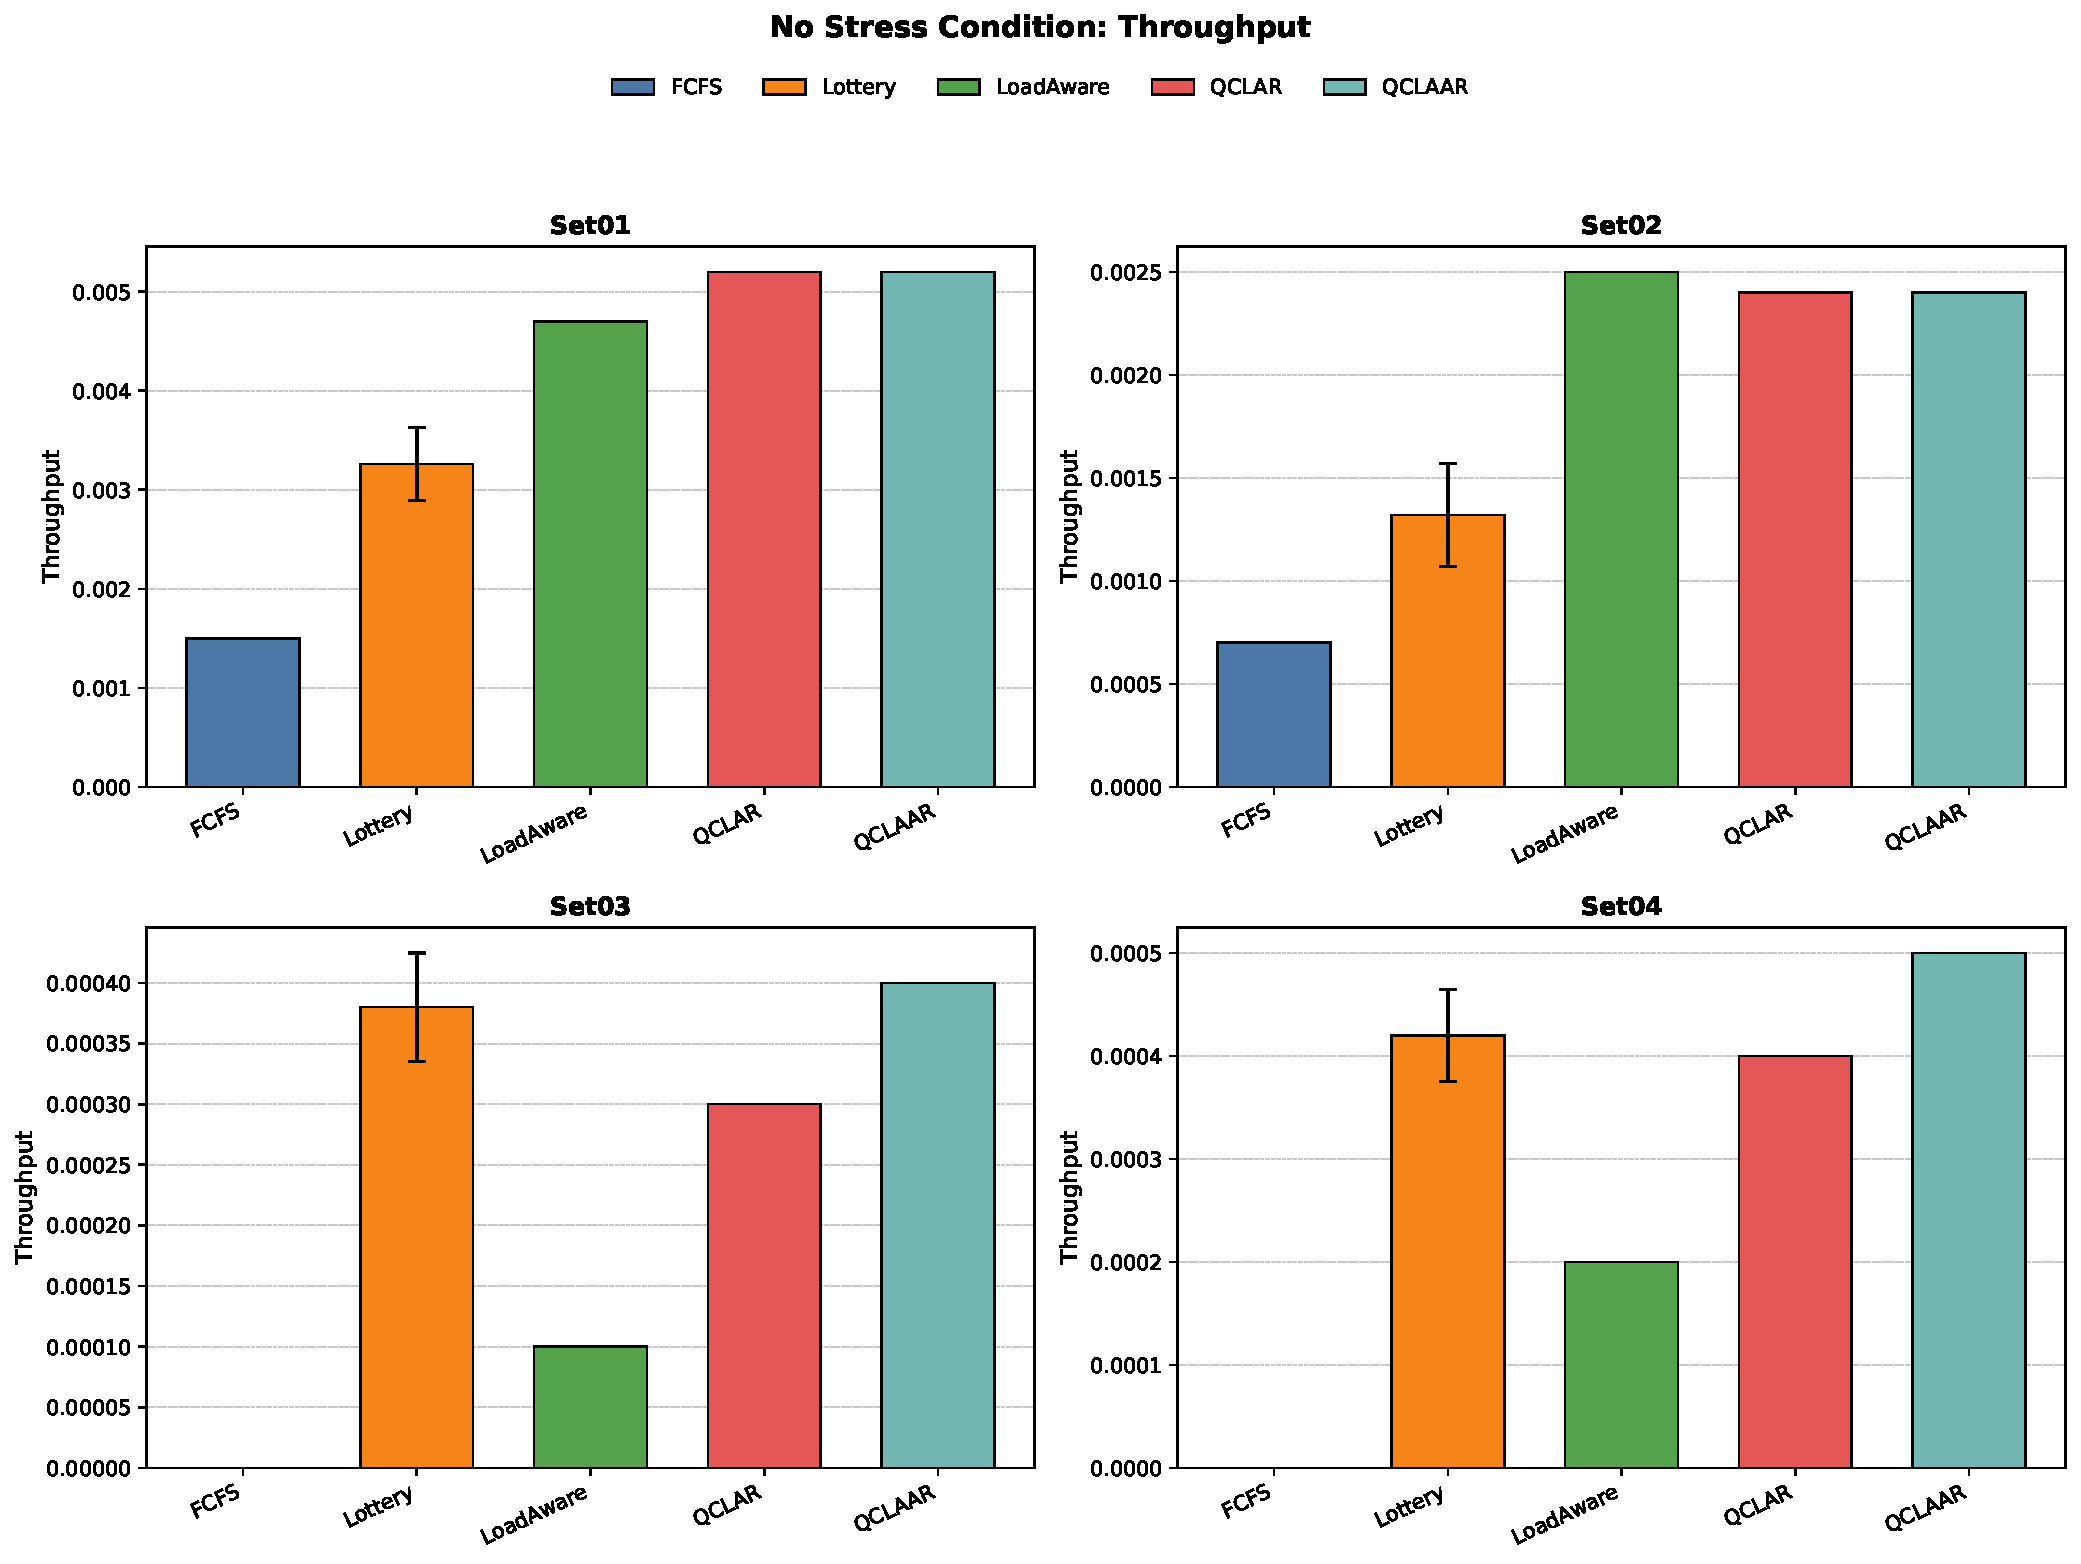
\includegraphics[width=0.95\linewidth]{Figure4_no_stress_throughput.pdf}
  \caption{Throughput under no-stress conditions.}
  \label{fig:thr-nostress}
\end{figure}

\begin{figure}[htbp]
  \centering
  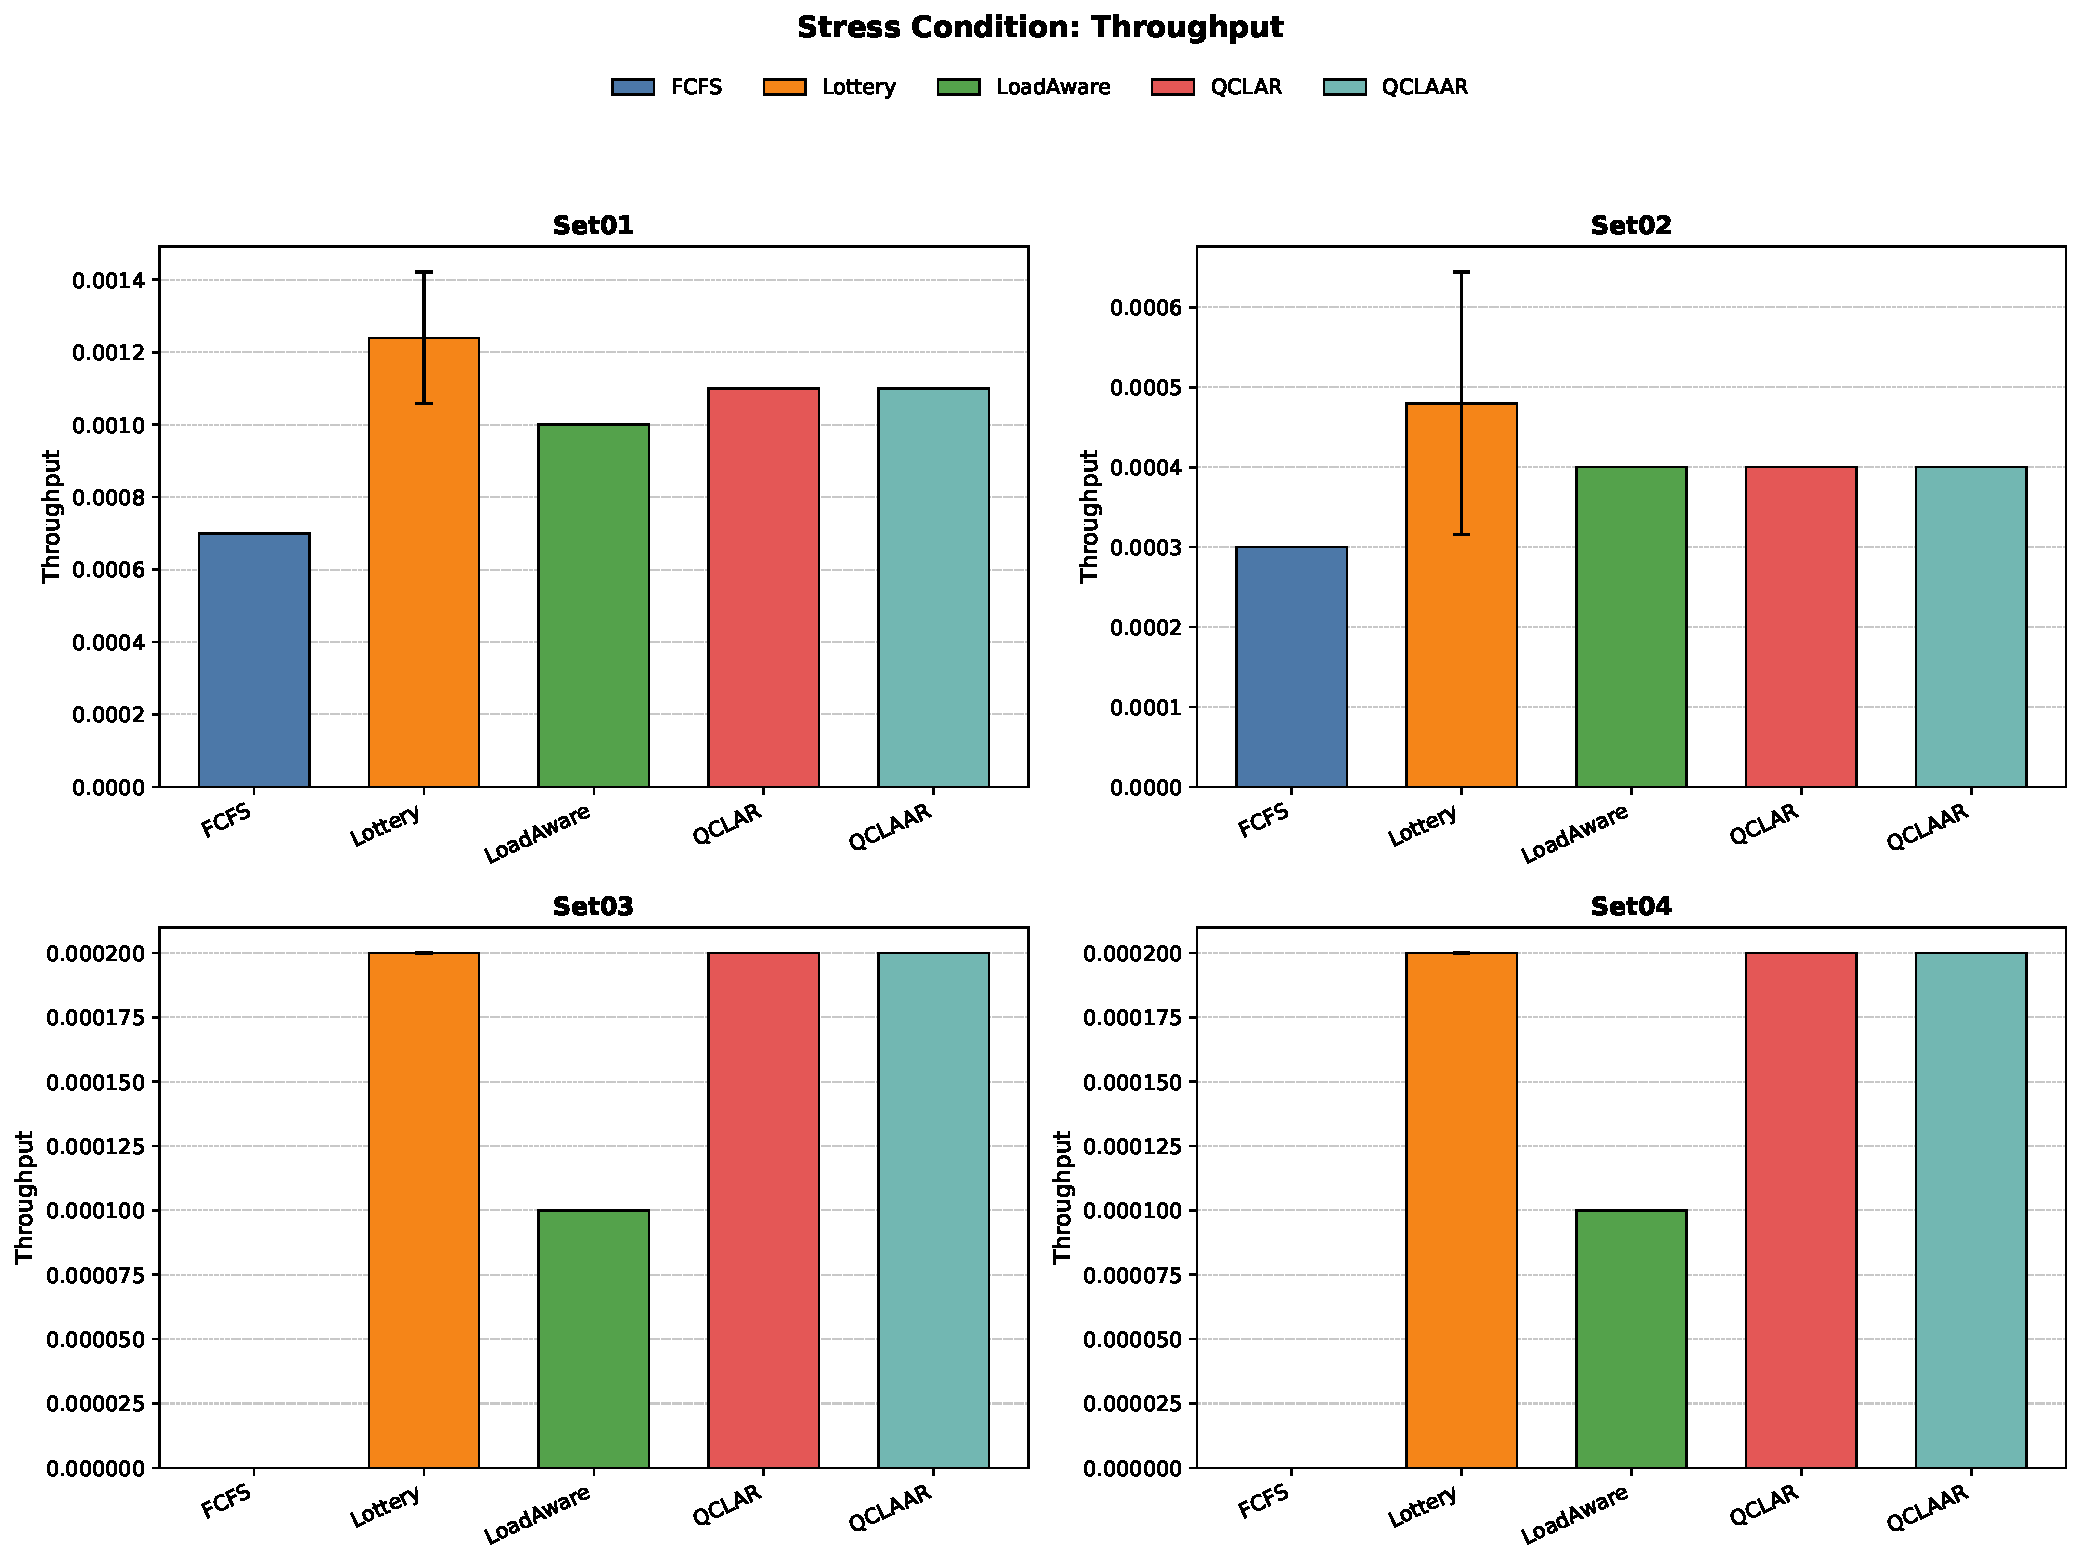
\includegraphics[width=0.95\linewidth]{Figure7_stress_throughput.pdf}
  \caption{Throughput under stress conditions.}
  \label{fig:thr-stress}
\end{figure}

\subsection{Stability and variability analysis}
\label{sec:variability}
The variation of \Lottery{}-based scheduling across repeated runs is shown in
Figure~\ref{fig:variability}. Variance grows sharply with workload size,
particularly for Set03 and Set04, indicating sensitivity to random selection
under heavy load. In contrast, the deterministic policies (\FCFS{},
\LoadAware{}, \QCLAR{}, and \QCLAAR{}) reproduce identical outcomes on every
execution. Although \Lottery{} is occasionally competitive, its lack of
predictability makes it unreliable for scheduling. These findings indicate that
capability-sensitive deterministic strategies offer a more robust alternative to
stochastic exploration in hybrid quantum scheduling.

\begin{figure}[htbp]
  \centering
  \begin{subfigure}[b]{0.49\linewidth}
    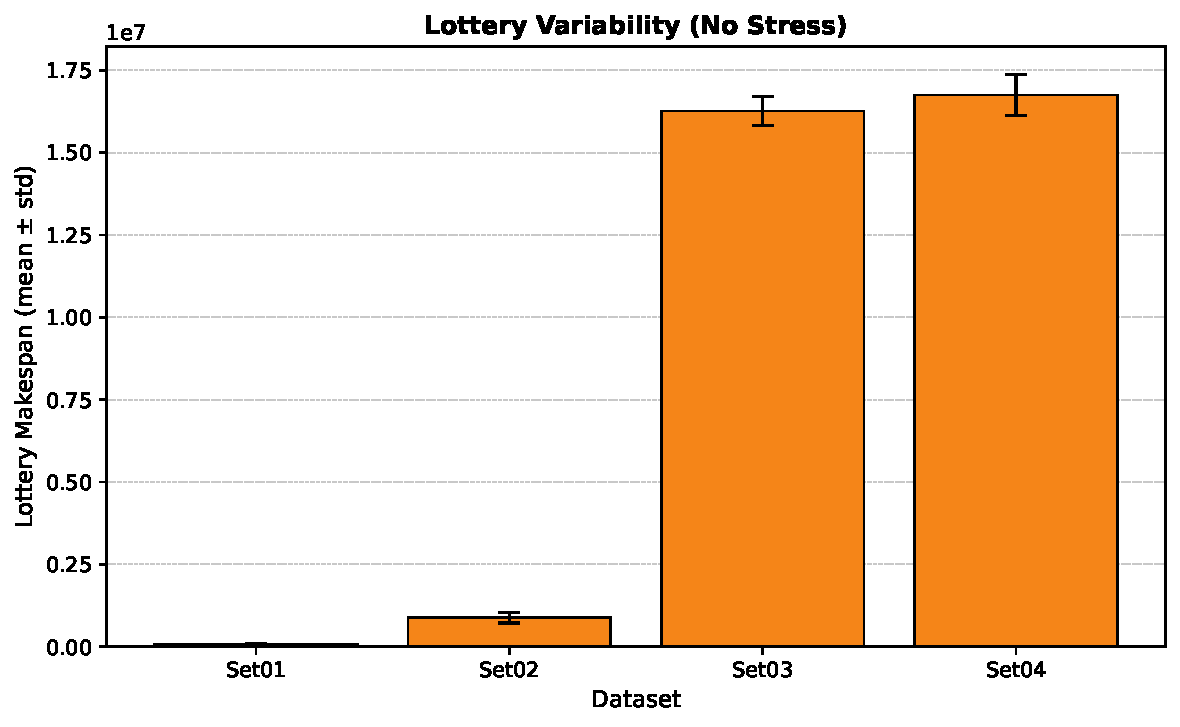
\includegraphics[width=\linewidth]{Figure8_lottery_variability_no_stress.pdf}
    \caption{No-stress condition}
    \label{fig:var-nostress}
  \end{subfigure}
  \hfill
  \begin{subfigure}[b]{0.49\linewidth}
    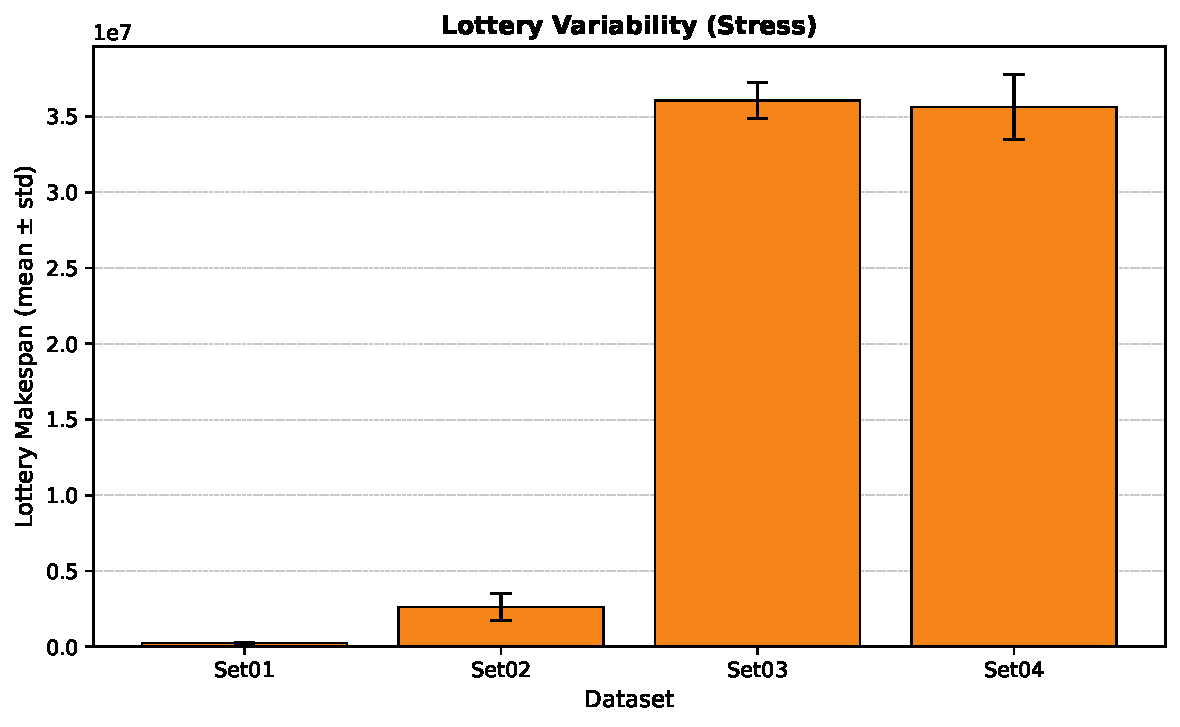
\includegraphics[width=\linewidth]{Figure8_lottery_variability_stress.pdf}
    \caption{Stress condition}
    \label{fig:var-stress}
  \end{subfigure}
  \caption{Lottery makespan variability across repeated runs
  (mean $\pm$ standard deviation).}
  \label{fig:variability}
\end{figure}

\subsection{Effect of the aging-inspired queue-pressure term}
\label{sec:aging}
Because \QCLAAR{} differs from \QCLAR{} only by the term $\lambda\hat{a}_j$, the
two policies isolate the contribution of queue-pressure awareness. Inspection of
the broker implementation, together with the five-run results in
Tables~\ref{tab:wait}--\ref{tab:throughput}, gives a complete account of what
this term does and does not achieve.

On Set01 and Set02 the two policies return identical values for every metric,
under both no-stress and stress conditions. This is a direct consequence of how
$\hat{a}_j$ is computed: the broker takes the waiting-list length of each
feasible candidate node and min--max normalises it across that candidate set at
the moment of scheduling. When every candidate has the same waiting-list length
--- which on Set01 and Set02 is true almost throughout, since these workloads
rarely leave more than one task queued at any single backend --- the
normalisation's range collapses to zero and the term is defined to return zero
for every candidate. It therefore drops out of the composite score identically,
and \QCLAAR{} reduces exactly to \QCLAR{} for these two datasets.

On the larger datasets, backends more often carry visibly different queue
lengths, so the term is active, and its effect depends on the regime. Under no
stress it helps: \QCLAAR{} improves on \QCLAR{} by 1.3\% and 1.2\% in waiting
time and by 6.9\% in makespan on Set03 and Set04. Under stress waiting time
still improves slightly (0.6\% and 2.0\%), but makespan worsens by 2.7\% and
3.2\%. The mechanism is visible in the term's definition: because $\hat{a}_j$
is a snapshot of the \emph{current} queue length rather than an accumulated
measure of how long any specific task has waited, it can repeatedly redirect
incoming tasks toward a momentarily short queue at a less capable backend. Under
stress this steers enough execution burden onto weaker candidates that the
schedule's tail lengthens, even as the average individual wait improves.

The aging-inspired term therefore does not deliver a uniform improvement, and at
the fixed weight $\lambda = 0.15$ it is inactive on light workloads (by
construction, since normalisation over an equal-valued candidate set is always
zero) and counterproductive for makespan under heavy load. Two concrete
modifications follow directly from this diagnosis and are natural next steps:
replacing the per-candidate min--max normalisation with a measure of absolute
queue length, so that the term remains non-zero even when candidates are tied;
and replacing the queue-length snapshot with the accumulated waiting time of
individual tasks, which is closer to aging in the conventional scheduling sense
and would not reward repeatedly redirecting new arrivals toward a momentarily
short queue. Whether either change, or a re-tuned $\lambda$, yields a consistent
benefit requires the sensitivity analysis identified in
Section~\ref{sec:limitations}.

\subsection{Comparative discussion}
The results support a narrower conclusion than a uniform ranking of policies.
\FCFS{} is dominated everywhere and is not a viable policy for this setting.
Beyond that, the ordering depends on workload scale, condition, and metric:
across the 24 combinations of three metrics, two conditions, and four datasets
in Tables~\ref{tab:wait}--\ref{tab:throughput}, the proposed policies win 16,
\LoadAware{} wins 3, and \Lottery{} wins 5.

The four small-dataset losses (all on Set02, under no stress) are narrow:
\LoadAware{} leads by 0.1\% in waiting time and 3.8\% in makespan and
throughput. Set01 is a partial exception to the small-dataset pattern --- while
its waiting-time margin is similarly negligible (0.8\%), \QCLAR{} leads
\LoadAware{} in makespan and throughput by roughly 10\%, a difference too large
to attribute to noise given the exact determinism confirmed across five runs
(Section~\ref{sec:variability}). Where the feasible set is homogeneous and
queues are short, predicted load captures most of the available signal, but not
all of it even on the smallest dataset tested.

On the large datasets (Set03, Set04), where backends differ substantially in
capability and tasks differ substantially in execution burden, the proposed
policies separate clearly from \LoadAware{} --- by roughly 25\% in waiting time
and 60\% in makespan under no stress. This is the regime the composite score was
designed for, and it is where the contribution of this work lies most clearly.

\Lottery{} occupies a distinct position, winning all 5 of its comparisons under
stress on makespan or throughput. It is competitive here because its
capability-weighted sampling captures part of the same signal the proposed
policies use explicitly. Its disadvantage is not mean performance but
dispersion: as Section~\ref{sec:variability} shows, its makespan standard
deviation reaches 2.12M on Set04 under stress, so any single run may land far
from the reported mean. For a production broker, a deterministic policy with a
slightly worse mean but reproducible behaviour is generally preferable to a
stochastic one whose realised performance cannot be predicted --- but this is an
argument about operational predictability, not about raw throughput.

\subsection{Limitations}
\label{sec:limitations}
The present study has several limitations. First, the evaluation is carried out
in a simulated environment, measuring scheduling behaviour at the system level
rather than on actual quantum hardware. Second, all five policies were executed
five times per dataset and condition; this confirmed that \FCFS{}, \LoadAware{},
\QCLAR{}, and \QCLAAR{} are exactly deterministic on a fixed workload instance
(zero variance across runs) and quantified \Lottery{}'s run-to-run variability
directly (Tables~\ref{tab:wait}--\ref{tab:throughput}), but all five runs reuse
the same four workload files, so this does not establish that the sub-percent
margins observed on Set02 would survive an independently drawn workload instance
of similar size and composition. Repeated runs over multiple independently
generated workload instances, with paired significance testing, would be
required before those specific margins are interpreted as a reliable ordering;
the 10\% margins observed on Set01 and the roughly 25--60\% margins on Set03 and
Set04 are large enough relative to the demonstrated run-to-run stability that
this concern applies mainly to Set02. Third, the weights $\alpha$, $\beta$,
$\gamma$, and $\lambda$ were selected empirically and held fixed; no sensitivity
analysis over the weight space was performed, so the extent to which the
reported results depend on this particular choice is unknown --- a question made
more pressing by the mixed behaviour of the queue-pressure term reported in
Section~\ref{sec:aging}. Fourth, \QCLAAR{} models aging through instantaneous
queue-length pressure rather than accumulated task waiting time, and
Section~\ref{sec:aging} identifies this as the likely cause of its inconsistent
effect on makespan. Finally, because the results are workload-sensitive,
relative performance trends may change under different workload distributions or
hardware settings, and the study does not model quantum noise dynamics or
hardware calibration, even though these influence scheduling behaviour in
practice. Despite these caveats, the controlled simulation environment permits
repeatable comparison of scheduling policies under identical execution
conditions, and the limitations above indicate clear avenues for further
testing on real-world quantum cloud architectures.

%=====================================================================
\section{Conclusion and Future Work}
\label{sec:conclusion}
%=====================================================================
This paper presents a broker-level scheduling model for hybrid quantum
edge--cloud systems, addressing the problem of capability- and queue-aware
backend selection over heterogeneous resources. Integrating the scheduling logic
into the iQuantum environment enabled uniform evaluation of baseline and
proposed policies at both the edge and cloud layers. The model was then extended
with two composite-score policies, \QCLAR{} and \QCLAAR{}, which incorporate
load state, execution burden, and backend capability; \QCLAAR{} additionally
includes an aging-inspired queue-pressure term. Results were verified directly
from five independent simulation runs per policy, dataset, and condition,
confirming that FCFS, LoadAware, QCLAR, and QCLAAR are exactly deterministic on
a fixed workload and quantifying Lottery's run-to-run variability. Across the
resulting 24 metric-dataset-condition comparisons, the proposed policies win
16, with the clearest advantage --- roughly 25\% in waiting time and 60\% in
makespan over LoadAware --- on the two large, heterogeneous datasets. On the
smaller datasets the picture is more qualified than a simple "no advantage"
conclusion: predicted load alone is close to sufficient on one dataset (LoadAware
leads QCLAR by under 4\%), but on the other, QCLAR still leads LoadAware in
makespan and throughput by roughly 10\% even though the candidate backends are
lightly loaded. The queue-pressure extension in QCLAAR proved beneficial for
waiting time and, under no stress, for makespan, but worsened makespan under
stress on the large datasets; inspecting the implementation traced this to the
term's use of an instantaneous, per-decision queue-length snapshot rather than
an accumulated measure of task waiting time, and to a normalisation that is
identically zero whenever candidate backends carry equal queue lengths. The
comparison of stochastic and deterministic policies further highlights that
reproducibility, rather than mean performance alone, is a relevant criterion in
scheduling design.

Future work includes revising the aging term to use accumulated task waiting
time or an unnormalised queue-pressure measure, so that it remains active and
beneficial under heavy load; a systematic sensitivity analysis over the
composite-score weights; evaluation on independently generated workload
instances to establish statistical significance for the narrower margins
observed here; adaptive or learning-based scheduling strategies; and performance
evaluation in larger, more realistic multi-datacenter deployments. Validation on
real-world quantum cloud systems offers a further opportunity to connect these
results with practice. Overall, this study demonstrates that broker-level
scheduling is an essential optimisation layer for next-generation hybrid quantum
systems, and that capability-aware routing is a promising model for the
reliable and efficient
management of quantum resources.

%=====================================================================
% Declarations
%=====================================================================
\section*{CRediT authorship contribution statement}
\textbf{First A. Author}: Conceptualization, Methodology, Software,
Investigation, Writing -- original draft.
\textbf{Second B. Author}: Validation, Formal analysis, Visualization,
Writing -- review \& editing.
\textbf{Third C. Author}: Supervision, Resources, Writing -- review \& editing.

\section*{Declaration of competing interest}
The authors declare that they have no known competing financial interests or
personal relationships that could have appeared to influence the work reported
in this paper.

\section*{Data availability}
Data will be made available on request.

\section*{Acknowledgements}
% TODO: add funding and acknowledgements, or delete this section.
The authors thank the anonymous reviewers for their constructive comments.

%=====================================================================
% References
%---------------------------------------------------------------------
% Bibliography data is in references.bib (all entries carry verified
% DOIs). Build sequence:
%     pdflatex main -> bibtex main -> pdflatex main -> pdflatex main
%
% To compile without BibTeX instead, replace the two lines below with:
%     % Fallback bibliography: the same 30 corrected references as an
% inline thebibliography environment, for compiling without BibTeX.
% To use, replace the \bibliographystyle/\bibliography lines in
% main.tex with:  % Fallback bibliography: the same 30 corrected references as an
% inline thebibliography environment, for compiling without BibTeX.
% To use, replace the \bibliographystyle/\bibliography lines in
% main.tex with:  % Fallback bibliography: the same 30 corrected references as an
% inline thebibliography environment, for compiling without BibTeX.
% To use, replace the \bibliographystyle/\bibliography lines in
% main.tex with:  \input{references-inline}

\begin{thebibliography}{30}

\bibitem{nguyen2024}
H.~T. Nguyen, M.~Usman, R.~Buyya,
iQuantum: A toolkit for modeling and simulation of quantum computing
environments,
Software: Practice and Experience 54~(6) (2024) 1141--1171.

\bibitem{calheiros2011}
R.~N. Calheiros, R.~Ranjan, A.~Beloglazov, C.~A.~F. De~Rose, R.~Buyya,
CloudSim: A toolkit for modeling and simulation of cloud computing environments
and evaluation of resource provisioning algorithms,
Software: Practice and Experience 41~(1) (2011) 23--50.

\bibitem{mahmud2022}
R.~Mahmud, S.~Pallewatta, M.~Goudarzi, R.~Buyya,
iFogSim2: An extended iFogSim simulator for mobility, clustering, and
microservice management in edge and fog computing environments,
Journal of Systems and Software 190 (2022) 111351.

\bibitem{preskill2018}
J.~Preskill,
Quantum computing in the NISQ era and beyond,
Quantum 2 (2018) 79.

\bibitem{nielsen2010}
M.~A. Nielsen, I.~L. Chuang,
Quantum Computation and Quantum Information,
Cambridge University Press, Cambridge, UK, 2010.

\bibitem{cross2019}
A.~W. Cross, L.~S. Bishop, S.~Sheldon, P.~D. Nation, J.~M. Gambetta,
Validating quantum computers using randomized model circuits,
Physical Review A 100~(3) (2019).

\bibitem{proctor2025}
T.~Proctor, K.~Young, A.~D. Baczewski, R.~Blume-Kohout,
Benchmarking quantum computers,
Nature Reviews Physics 7 (2025) 105--118.

\bibitem{magesan2011}
E.~Magesan, J.~M. Gambetta, J.~Emerson,
Scalable and robust randomized benchmarking of quantum processes,
Physical Review Letters 106~(18) (2011).

\bibitem{magesan2012}
E.~Magesan, J.~M. Gambetta, B.~R. Johnson, C.~A. Ryan, J.~M. Chow,
S.~T. Merkel, M.~P. da~Silva, G.~A. Keefe, M.~B. Rothwell, T.~A. Ohki,
M.~B. Ketchen, J.~M. Steffen,
Efficient measurement of quantum gate error by interleaved randomized
benchmarking,
Physical Review Letters 109~(8) (2012).

\bibitem{yao2025}
G.~Yao, L.~Gupta,
A benchmarking framework for hybrid quantum--classical edge-cloud computing
systems,
Applied Sciences 15 (2025) 10245.

\bibitem{furutanpey2023}
A.~Furutanpey, J.~Barzen, M.~Bechtold, S.~Dustdar, F.~Leymann, P.~Raith,
F.~Truger,
Architectural vision for quantum computing in the edge-cloud continuum,
in: Proc. IEEE International Conference on Quantum Software (QSW), 2023,
pp. 88--103.

\bibitem{mastroianni2023}
C.~Mastroianni, L.~Scarcello, A.~Vinci,
Quantum computing management of a cloud/edge architecture,
in: Proc. ACM International Conference on Computing Frontiers (CF), 2023,
pp. 193--196.

\bibitem{xu2025}
M.~Xu, D.~Niyato, J.~Kang, Z.~Xiong, M.~Chen, D.~I. Kim, X.~Shen,
Hybrid reinforcement learning-based sustainable multi-user computation
offloading for mobile edge-quantum computing,
arXiv:2504.08134 (2025).

\bibitem{huang2024}
S.~Huang, L.~Wang, X.~Wang, B.~Tan, W.~Ni, K.-K. Wong,
Edge intelligence in satellite-terrestrial networks with hybrid quantum
computing,
arXiv:2409.19869 (2024).

\bibitem{satya2017}
M.~Satyanarayanan,
The emergence of edge computing,
Computer 50~(1) (2017) 30--39.

\bibitem{shi2016}
W.~Shi, J.~Cao, Q.~Zhang, Y.~Li, L.~Xu,
Edge computing: Vision and challenges,
IEEE Internet of Things Journal 3~(5) (2016) 637--646.

\bibitem{mao2017}
Y.~Mao, C.~You, J.~Zhang, K.~Huang, K.~B. Letaief,
A survey on mobile edge computing: The communication perspective,
IEEE Communications Surveys \& Tutorials 19~(4) (2017) 2322--2358.

\bibitem{abbas2018}
N.~Abbas, Y.~Zhang, A.~Taherkordi, T.~Skeie,
Mobile edge computing: A survey,
IEEE Internet of Things Journal 5~(1) (2018) 450--465.

\bibitem{leymann2020}
F.~Leymann, J.~Barzen, M.~Falkenthal, D.~Vietz, B.~Weder, K.~Wild,
Quantum in the cloud: Application potentials and research opportunities,
in: Proc. 10th International Conference on Cloud Computing and Services Science
(CLOSER), SciTePress, 2020, pp. 9--24.

\bibitem{weder2021a}
B.~Weder, J.~Barzen, F.~Leymann, M.~Salm, D.~Vietz,
The quantum software lifecycle,
in: Proc. 1st ACM SIGSOFT International Workshop on Architectures and Paradigms
for Engineering Quantum Software (APEQS), ACM, 2020, pp. 2--9.

\bibitem{weder2021b}
% REPLACED: the entry previously here ("Quantum application archives:
% Supporting the reuse of quantum applications") could not be located in any
% bibliographic database and appears not to exist. Substituted with a real,
% topically adjacent paper by the same group -- VERIFY this is what you meant
% to cite, or delete this entry (it is currently uncited in the text).
B.~Weder, J.~Barzen, F.~Leymann, M.~Zimmermann,
Hybrid quantum applications need two orchestrations in superposition: A software
architecture perspective,
in: Proc. 18th IEEE International Conference on Web Services (ICWS), IEEE, 2021.

\bibitem{wild2021}
K.~Wild, U.~Breitenb\"{u}cher, L.~Harzenetter, F.~Leymann, D.~Vietz,
M.~Zimmermann,
TOSCA4QC: Two modeling styles for TOSCA to automate the deployment and
orchestration of quantum applications,
in: Proc. 24th IEEE International Enterprise Distributed Object Computing
Conference (EDOC), IEEE, 2020, pp. 125--134.

\bibitem{garcia2022}
J.~Garcia-Alonso, J.~Rojo, D.~Valencia, E.~Moguel, J.~Berrocal, J.~M. Murillo,
Quantum software as a service through a quantum API gateway,
IEEE Internet Computing 26~(1) (2022) 34--41.

\bibitem{beisel2023}
M.~Beisel, J.~Barzen, S.~Garhofer, F.~Leymann, F.~Truger, B.~Weder,
V.~Yussupov,
Quokka: A service ecosystem for workflow-based execution of variational quantum
algorithms,
in: Service-Oriented Computing -- ICSOC 2022 Workshops, Vol. 13821 of LNCS,
Springer, 2023, pp. 369--373.

\bibitem{quetschlich2023}
N.~Quetschlich, L.~Burgholzer, R.~Wille,
MQT Bench: Benchmarking software and design automation tools for quantum
computing,
Quantum 7 (2023) 1062.

\bibitem{li2020}
A.~Li, S.~Stein, S.~Krishnamoorthy, J.~Ang,
QASMBench: A low-level quantum benchmark suite for NISQ evaluation and
simulation,
ACM Transactions on Quantum Computing 4~(2) (2023) 1--26.

\bibitem{tomesh2022}
T.~Tomesh, P.~Gokhale, V.~Omole, G.~S. Ravi, K.~N. Smith, J.~Viszlai,
X.-C. Wu, N.~Hardavellas, M.~R. Martonosi, F.~T. Chong,
SupermarQ: A scalable quantum benchmark suite,
in: Proc. IEEE International Symposium on High-Performance Computer
Architecture (HPCA), IEEE, 2022, pp. 587--603.

\bibitem{finzgar2024}
J.~R. Fin\v{z}gar, P.~Ross, L.~H\"{o}lscher, J.~Klepsch, A.~Luckow,
QUARK: A framework for quantum computing application benchmarking,
in: Proc. IEEE International Conference on Quantum Computing and Engineering
(QCE), IEEE, 2022, pp. 226--237.

\bibitem{farhi2014}
E.~Farhi, J.~Goldstone, S.~Gutmann,
A quantum approximate optimization algorithm,
arXiv:1411.4028 (2014).

\bibitem{cerezo2021}
M.~Cerezo, A.~Arrasmith, R.~Babbush, S.~C. Benjamin, S.~Endo, K.~Fujii,
J.~R. McClean, K.~Mitarai, X.~Yuan, L.~Cincio, P.~J. Coles,
Variational quantum algorithms,
Nature Reviews Physics 3 (2021) 625--644.

\end{thebibliography}


\begin{thebibliography}{30}

\bibitem{nguyen2024}
H.~T. Nguyen, M.~Usman, R.~Buyya,
iQuantum: A toolkit for modeling and simulation of quantum computing
environments,
Software: Practice and Experience 54~(6) (2024) 1141--1171.

\bibitem{calheiros2011}
R.~N. Calheiros, R.~Ranjan, A.~Beloglazov, C.~A.~F. De~Rose, R.~Buyya,
CloudSim: A toolkit for modeling and simulation of cloud computing environments
and evaluation of resource provisioning algorithms,
Software: Practice and Experience 41~(1) (2011) 23--50.

\bibitem{mahmud2022}
R.~Mahmud, S.~Pallewatta, M.~Goudarzi, R.~Buyya,
iFogSim2: An extended iFogSim simulator for mobility, clustering, and
microservice management in edge and fog computing environments,
Journal of Systems and Software 190 (2022) 111351.

\bibitem{preskill2018}
J.~Preskill,
Quantum computing in the NISQ era and beyond,
Quantum 2 (2018) 79.

\bibitem{nielsen2010}
M.~A. Nielsen, I.~L. Chuang,
Quantum Computation and Quantum Information,
Cambridge University Press, Cambridge, UK, 2010.

\bibitem{cross2019}
A.~W. Cross, L.~S. Bishop, S.~Sheldon, P.~D. Nation, J.~M. Gambetta,
Validating quantum computers using randomized model circuits,
Physical Review A 100~(3) (2019).

\bibitem{proctor2025}
T.~Proctor, K.~Young, A.~D. Baczewski, R.~Blume-Kohout,
Benchmarking quantum computers,
Nature Reviews Physics 7 (2025) 105--118.

\bibitem{magesan2011}
E.~Magesan, J.~M. Gambetta, J.~Emerson,
Scalable and robust randomized benchmarking of quantum processes,
Physical Review Letters 106~(18) (2011).

\bibitem{magesan2012}
E.~Magesan, J.~M. Gambetta, B.~R. Johnson, C.~A. Ryan, J.~M. Chow,
S.~T. Merkel, M.~P. da~Silva, G.~A. Keefe, M.~B. Rothwell, T.~A. Ohki,
M.~B. Ketchen, J.~M. Steffen,
Efficient measurement of quantum gate error by interleaved randomized
benchmarking,
Physical Review Letters 109~(8) (2012).

\bibitem{yao2025}
G.~Yao, L.~Gupta,
A benchmarking framework for hybrid quantum--classical edge-cloud computing
systems,
Applied Sciences 15 (2025) 10245.

\bibitem{furutanpey2023}
A.~Furutanpey, J.~Barzen, M.~Bechtold, S.~Dustdar, F.~Leymann, P.~Raith,
F.~Truger,
Architectural vision for quantum computing in the edge-cloud continuum,
in: Proc. IEEE International Conference on Quantum Software (QSW), 2023,
pp. 88--103.

\bibitem{mastroianni2023}
C.~Mastroianni, L.~Scarcello, A.~Vinci,
Quantum computing management of a cloud/edge architecture,
in: Proc. ACM International Conference on Computing Frontiers (CF), 2023,
pp. 193--196.

\bibitem{xu2025}
M.~Xu, D.~Niyato, J.~Kang, Z.~Xiong, M.~Chen, D.~I. Kim, X.~Shen,
Hybrid reinforcement learning-based sustainable multi-user computation
offloading for mobile edge-quantum computing,
arXiv:2504.08134 (2025).

\bibitem{huang2024}
S.~Huang, L.~Wang, X.~Wang, B.~Tan, W.~Ni, K.-K. Wong,
Edge intelligence in satellite-terrestrial networks with hybrid quantum
computing,
arXiv:2409.19869 (2024).

\bibitem{satya2017}
M.~Satyanarayanan,
The emergence of edge computing,
Computer 50~(1) (2017) 30--39.

\bibitem{shi2016}
W.~Shi, J.~Cao, Q.~Zhang, Y.~Li, L.~Xu,
Edge computing: Vision and challenges,
IEEE Internet of Things Journal 3~(5) (2016) 637--646.

\bibitem{mao2017}
Y.~Mao, C.~You, J.~Zhang, K.~Huang, K.~B. Letaief,
A survey on mobile edge computing: The communication perspective,
IEEE Communications Surveys \& Tutorials 19~(4) (2017) 2322--2358.

\bibitem{abbas2018}
N.~Abbas, Y.~Zhang, A.~Taherkordi, T.~Skeie,
Mobile edge computing: A survey,
IEEE Internet of Things Journal 5~(1) (2018) 450--465.

\bibitem{leymann2020}
F.~Leymann, J.~Barzen, M.~Falkenthal, D.~Vietz, B.~Weder, K.~Wild,
Quantum in the cloud: Application potentials and research opportunities,
in: Proc. 10th International Conference on Cloud Computing and Services Science
(CLOSER), SciTePress, 2020, pp. 9--24.

\bibitem{weder2021a}
B.~Weder, J.~Barzen, F.~Leymann, M.~Salm, D.~Vietz,
The quantum software lifecycle,
in: Proc. 1st ACM SIGSOFT International Workshop on Architectures and Paradigms
for Engineering Quantum Software (APEQS), ACM, 2020, pp. 2--9.

\bibitem{weder2021b}
% REPLACED: the entry previously here ("Quantum application archives:
% Supporting the reuse of quantum applications") could not be located in any
% bibliographic database and appears not to exist. Substituted with a real,
% topically adjacent paper by the same group -- VERIFY this is what you meant
% to cite, or delete this entry (it is currently uncited in the text).
B.~Weder, J.~Barzen, F.~Leymann, M.~Zimmermann,
Hybrid quantum applications need two orchestrations in superposition: A software
architecture perspective,
in: Proc. 18th IEEE International Conference on Web Services (ICWS), IEEE, 2021.

\bibitem{wild2021}
K.~Wild, U.~Breitenb\"{u}cher, L.~Harzenetter, F.~Leymann, D.~Vietz,
M.~Zimmermann,
TOSCA4QC: Two modeling styles for TOSCA to automate the deployment and
orchestration of quantum applications,
in: Proc. 24th IEEE International Enterprise Distributed Object Computing
Conference (EDOC), IEEE, 2020, pp. 125--134.

\bibitem{garcia2022}
J.~Garcia-Alonso, J.~Rojo, D.~Valencia, E.~Moguel, J.~Berrocal, J.~M. Murillo,
Quantum software as a service through a quantum API gateway,
IEEE Internet Computing 26~(1) (2022) 34--41.

\bibitem{beisel2023}
M.~Beisel, J.~Barzen, S.~Garhofer, F.~Leymann, F.~Truger, B.~Weder,
V.~Yussupov,
Quokka: A service ecosystem for workflow-based execution of variational quantum
algorithms,
in: Service-Oriented Computing -- ICSOC 2022 Workshops, Vol. 13821 of LNCS,
Springer, 2023, pp. 369--373.

\bibitem{quetschlich2023}
N.~Quetschlich, L.~Burgholzer, R.~Wille,
MQT Bench: Benchmarking software and design automation tools for quantum
computing,
Quantum 7 (2023) 1062.

\bibitem{li2020}
A.~Li, S.~Stein, S.~Krishnamoorthy, J.~Ang,
QASMBench: A low-level quantum benchmark suite for NISQ evaluation and
simulation,
ACM Transactions on Quantum Computing 4~(2) (2023) 1--26.

\bibitem{tomesh2022}
T.~Tomesh, P.~Gokhale, V.~Omole, G.~S. Ravi, K.~N. Smith, J.~Viszlai,
X.-C. Wu, N.~Hardavellas, M.~R. Martonosi, F.~T. Chong,
SupermarQ: A scalable quantum benchmark suite,
in: Proc. IEEE International Symposium on High-Performance Computer
Architecture (HPCA), IEEE, 2022, pp. 587--603.

\bibitem{finzgar2024}
J.~R. Fin\v{z}gar, P.~Ross, L.~H\"{o}lscher, J.~Klepsch, A.~Luckow,
QUARK: A framework for quantum computing application benchmarking,
in: Proc. IEEE International Conference on Quantum Computing and Engineering
(QCE), IEEE, 2022, pp. 226--237.

\bibitem{farhi2014}
E.~Farhi, J.~Goldstone, S.~Gutmann,
A quantum approximate optimization algorithm,
arXiv:1411.4028 (2014).

\bibitem{cerezo2021}
M.~Cerezo, A.~Arrasmith, R.~Babbush, S.~C. Benjamin, S.~Endo, K.~Fujii,
J.~R. McClean, K.~Mitarai, X.~Yuan, L.~Cincio, P.~J. Coles,
Variational quantum algorithms,
Nature Reviews Physics 3 (2021) 625--644.

\end{thebibliography}


\begin{thebibliography}{30}

\bibitem{nguyen2024}
H.~T. Nguyen, M.~Usman, R.~Buyya,
iQuantum: A toolkit for modeling and simulation of quantum computing
environments,
Software: Practice and Experience 54~(6) (2024) 1141--1171.

\bibitem{calheiros2011}
R.~N. Calheiros, R.~Ranjan, A.~Beloglazov, C.~A.~F. De~Rose, R.~Buyya,
CloudSim: A toolkit for modeling and simulation of cloud computing environments
and evaluation of resource provisioning algorithms,
Software: Practice and Experience 41~(1) (2011) 23--50.

\bibitem{mahmud2022}
R.~Mahmud, S.~Pallewatta, M.~Goudarzi, R.~Buyya,
iFogSim2: An extended iFogSim simulator for mobility, clustering, and
microservice management in edge and fog computing environments,
Journal of Systems and Software 190 (2022) 111351.

\bibitem{preskill2018}
J.~Preskill,
Quantum computing in the NISQ era and beyond,
Quantum 2 (2018) 79.

\bibitem{nielsen2010}
M.~A. Nielsen, I.~L. Chuang,
Quantum Computation and Quantum Information,
Cambridge University Press, Cambridge, UK, 2010.

\bibitem{cross2019}
A.~W. Cross, L.~S. Bishop, S.~Sheldon, P.~D. Nation, J.~M. Gambetta,
Validating quantum computers using randomized model circuits,
Physical Review A 100~(3) (2019).

\bibitem{proctor2025}
T.~Proctor, K.~Young, A.~D. Baczewski, R.~Blume-Kohout,
Benchmarking quantum computers,
Nature Reviews Physics 7 (2025) 105--118.

\bibitem{magesan2011}
E.~Magesan, J.~M. Gambetta, J.~Emerson,
Scalable and robust randomized benchmarking of quantum processes,
Physical Review Letters 106~(18) (2011).

\bibitem{magesan2012}
E.~Magesan, J.~M. Gambetta, B.~R. Johnson, C.~A. Ryan, J.~M. Chow,
S.~T. Merkel, M.~P. da~Silva, G.~A. Keefe, M.~B. Rothwell, T.~A. Ohki,
M.~B. Ketchen, J.~M. Steffen,
Efficient measurement of quantum gate error by interleaved randomized
benchmarking,
Physical Review Letters 109~(8) (2012).

\bibitem{yao2025}
G.~Yao, L.~Gupta,
A benchmarking framework for hybrid quantum--classical edge-cloud computing
systems,
Applied Sciences 15 (2025) 10245.

\bibitem{furutanpey2023}
A.~Furutanpey, J.~Barzen, M.~Bechtold, S.~Dustdar, F.~Leymann, P.~Raith,
F.~Truger,
Architectural vision for quantum computing in the edge-cloud continuum,
in: Proc. IEEE International Conference on Quantum Software (QSW), 2023,
pp. 88--103.

\bibitem{mastroianni2023}
C.~Mastroianni, L.~Scarcello, A.~Vinci,
Quantum computing management of a cloud/edge architecture,
in: Proc. ACM International Conference on Computing Frontiers (CF), 2023,
pp. 193--196.

\bibitem{xu2025}
M.~Xu, D.~Niyato, J.~Kang, Z.~Xiong, M.~Chen, D.~I. Kim, X.~Shen,
Hybrid reinforcement learning-based sustainable multi-user computation
offloading for mobile edge-quantum computing,
arXiv:2504.08134 (2025).

\bibitem{huang2024}
S.~Huang, L.~Wang, X.~Wang, B.~Tan, W.~Ni, K.-K. Wong,
Edge intelligence in satellite-terrestrial networks with hybrid quantum
computing,
arXiv:2409.19869 (2024).

\bibitem{satya2017}
M.~Satyanarayanan,
The emergence of edge computing,
Computer 50~(1) (2017) 30--39.

\bibitem{shi2016}
W.~Shi, J.~Cao, Q.~Zhang, Y.~Li, L.~Xu,
Edge computing: Vision and challenges,
IEEE Internet of Things Journal 3~(5) (2016) 637--646.

\bibitem{mao2017}
Y.~Mao, C.~You, J.~Zhang, K.~Huang, K.~B. Letaief,
A survey on mobile edge computing: The communication perspective,
IEEE Communications Surveys \& Tutorials 19~(4) (2017) 2322--2358.

\bibitem{abbas2018}
N.~Abbas, Y.~Zhang, A.~Taherkordi, T.~Skeie,
Mobile edge computing: A survey,
IEEE Internet of Things Journal 5~(1) (2018) 450--465.

\bibitem{leymann2020}
F.~Leymann, J.~Barzen, M.~Falkenthal, D.~Vietz, B.~Weder, K.~Wild,
Quantum in the cloud: Application potentials and research opportunities,
in: Proc. 10th International Conference on Cloud Computing and Services Science
(CLOSER), SciTePress, 2020, pp. 9--24.

\bibitem{weder2021a}
B.~Weder, J.~Barzen, F.~Leymann, M.~Salm, D.~Vietz,
The quantum software lifecycle,
in: Proc. 1st ACM SIGSOFT International Workshop on Architectures and Paradigms
for Engineering Quantum Software (APEQS), ACM, 2020, pp. 2--9.

\bibitem{weder2021b}
% REPLACED: the entry previously here ("Quantum application archives:
% Supporting the reuse of quantum applications") could not be located in any
% bibliographic database and appears not to exist. Substituted with a real,
% topically adjacent paper by the same group -- VERIFY this is what you meant
% to cite, or delete this entry (it is currently uncited in the text).
B.~Weder, J.~Barzen, F.~Leymann, M.~Zimmermann,
Hybrid quantum applications need two orchestrations in superposition: A software
architecture perspective,
in: Proc. 18th IEEE International Conference on Web Services (ICWS), IEEE, 2021.

\bibitem{wild2021}
K.~Wild, U.~Breitenb\"{u}cher, L.~Harzenetter, F.~Leymann, D.~Vietz,
M.~Zimmermann,
TOSCA4QC: Two modeling styles for TOSCA to automate the deployment and
orchestration of quantum applications,
in: Proc. 24th IEEE International Enterprise Distributed Object Computing
Conference (EDOC), IEEE, 2020, pp. 125--134.

\bibitem{garcia2022}
J.~Garcia-Alonso, J.~Rojo, D.~Valencia, E.~Moguel, J.~Berrocal, J.~M. Murillo,
Quantum software as a service through a quantum API gateway,
IEEE Internet Computing 26~(1) (2022) 34--41.

\bibitem{beisel2023}
M.~Beisel, J.~Barzen, S.~Garhofer, F.~Leymann, F.~Truger, B.~Weder,
V.~Yussupov,
Quokka: A service ecosystem for workflow-based execution of variational quantum
algorithms,
in: Service-Oriented Computing -- ICSOC 2022 Workshops, Vol. 13821 of LNCS,
Springer, 2023, pp. 369--373.

\bibitem{quetschlich2023}
N.~Quetschlich, L.~Burgholzer, R.~Wille,
MQT Bench: Benchmarking software and design automation tools for quantum
computing,
Quantum 7 (2023) 1062.

\bibitem{li2020}
A.~Li, S.~Stein, S.~Krishnamoorthy, J.~Ang,
QASMBench: A low-level quantum benchmark suite for NISQ evaluation and
simulation,
ACM Transactions on Quantum Computing 4~(2) (2023) 1--26.

\bibitem{tomesh2022}
T.~Tomesh, P.~Gokhale, V.~Omole, G.~S. Ravi, K.~N. Smith, J.~Viszlai,
X.-C. Wu, N.~Hardavellas, M.~R. Martonosi, F.~T. Chong,
SupermarQ: A scalable quantum benchmark suite,
in: Proc. IEEE International Symposium on High-Performance Computer
Architecture (HPCA), IEEE, 2022, pp. 587--603.

\bibitem{finzgar2024}
J.~R. Fin\v{z}gar, P.~Ross, L.~H\"{o}lscher, J.~Klepsch, A.~Luckow,
QUARK: A framework for quantum computing application benchmarking,
in: Proc. IEEE International Conference on Quantum Computing and Engineering
(QCE), IEEE, 2022, pp. 226--237.

\bibitem{farhi2014}
E.~Farhi, J.~Goldstone, S.~Gutmann,
A quantum approximate optimization algorithm,
arXiv:1411.4028 (2014).

\bibitem{cerezo2021}
M.~Cerezo, A.~Arrasmith, R.~Babbush, S.~C. Benjamin, S.~Endo, K.~Fujii,
J.~R. McClean, K.~Mitarai, X.~Yuan, L.~Cincio, P.~J. Coles,
Variational quantum algorithms,
Nature Reviews Physics 3 (2021) 625--644.

\end{thebibliography}

% which pulls in the identical reference list as a plain
% thebibliography environment.
%=====================================================================
\bibliographystyle{elsarticle-num}
\bibliography{references}

\end{document}
